% ***************************************************************************************************
%
%	Szablon pracy magisterskiej dla Politechniki Wrocławskiej w wersji dwustronnej.
%	Autor:	Tomasz Strzałka
%
% ***************************************************************************************************

% Styl dwustronny z domyślną wielkością czcionki 10pt oraz oddzieloną stroną tytułową (titlepage).
% Domyślnie rodziały rozpoczynają się na stronie prawej (openright).
\documentclass{book}
% ***************************************************************************************************
% Ustawienia języka
% ***************************************************************************************************

% Podstawowe ustawienia języka, według którego formatowany będzie dokument
\usepackage[polish]{babel}

% Pakiet babel dla polskiego języka powoduje konflikt z pakietem amssymb.
% Polecenie '\lll' definiują oba pakiety - porządana jest druga definicja.
\let\lll\undefined

% W przypadku wielojęzykowości ustawia główny język dokumentu
\selectlanguage{polish}

% Kodowanie dokumentu
\usepackage[utf8]{inputenc}

% Dowolny rozmiar czcionek, kodowanie znaków
\usepackage{lmodern}

% Polskie wcięcia akapitów
\usepackage{indentfirst}

% Polskie łamanie wyrazów
\usepackage[plmath]{polski}

% Przecinek w wyrażeniach matematycznych zamiast kropki
\usepackage{icomma}

% Polskie formatowanie typograficzne
\frenchspacing

% Zapewnia liczne usprawnienia wyświetlania i organizacji matematycznych formuł. 
\usepackage{amsmath}

% Wprowadza rozszerzony zestaw symboli m.in. \leadsto
\usepackage{amssymb}

% Dodatkowa, ,,kręcona'' czcionka matematyczna
\usepackage{mathrsfs}

% Dodatkowe wsparcie dla środowiska mathbb, które nie wspiera domyślnie cyfr (\mathbb{})
\usepackage{bbold}

% Fixes/improves amsmath
\usepackage{mathtools}

% ***************************************************************************************************
% Kolory  
% ***************************************************************************************************

% Umożliwia kolorowanie poszczególnych komórek tabeli
\usepackage[table]{xcolor}% http://ctan.org/pkg/

% Umożliwia łatwą zmianę koloru linii w tabeli
\usepackage{tabu}

% Umożliwia rozszerzoną kontrolę nad kolorami.
\usepackage{xcolor}

\usepackage{float}

% Definicje kolorów
\definecolor{lgray}{HTML}{9F9F9F}
\definecolor{dgray}{HTML}{5F5F5F}
% lgray				-	nazwa nowo zdefiniowanego koloru
% HTML				-	model kolorów
% CCCCCC			-	wartość koloru zgodna z modelem

% ***************************************************************************************************
% Algorytmy 
% ***************************************************************************************************

% Udostępnia środowisko do konstruowania pseudokodów
\usepackage[ruled,vlined,linesnumbered,longend,algochapter]{algorithm2e}
% ruled	- poziome kreski na początku i końcu algorytmu, podpis na górze oddzielony również kreską poziomą
% vlined - pionowe kreski łączące początek polecenia z jego końcem
% linesnumbered	- numerowanie kolejnych wierszy algorytmu
% longend - długie końcówki np. ifend, forend itd.
% algochapter - numeracja z rozdziałami

% Zamiana nazwy środowiska z domyślnej "Algorithm X" na "Pseudokod X"
\newenvironment{pseudokod}[1][htb]{
	\renewcommand{\algorithmcfname}{Pseudokod}
	\begin{algorithm}[#1]%
	}{
\end{algorithm}
}

% Zmiana rozmiaru komentarzy
\newcommand\algcomment[1]{
	\footnotesize{#1}
}

% Ustawienie zadanego stylu dla komentarzy
\SetCommentSty{algcomment}

% Wyśrodkowana tylda
\usepackage{textcomp}%
\newcommand{\textapprox}{\raisebox{0.5ex}{\texttildelow}}

% Listowanie kodów źródłowych
\usepackage{listings} 
\renewcommand{\lstlistingname}{Kod źródłowy} % Polska nazwa listingu

% Definicje dla listingu JSON
\colorlet{punct}{red!60!black}
\definecolor{background}{HTML}{EEEEEE}
\definecolor{delim}{RGB}{20,105,176}
\colorlet{numb}{magenta!60!black}

\lstdefinelanguage{json}{
    basicstyle=\normalfont\ttfamily,
    numbers=left,
    numberstyle=\scriptsize,
    stepnumber=1,
    numbersep=8pt,
    showstringspaces=false,
    breaklines=true,
    frame=lines,
    backgroundcolor=\color{background},
    literate=
     *{0}{{{\color{numb}0}}}{1}
      {1}{{{\color{numb}1}}}{1}
      {2}{{{\color{numb}2}}}{1}
      {3}{{{\color{numb}3}}}{1}
      {4}{{{\color{numb}4}}}{1}
      {5}{{{\color{numb}5}}}{1}
      {6}{{{\color{numb}6}}}{1}
      {7}{{{\color{numb}7}}}{1}
      {8}{{{\color{numb}8}}}{1}
      {9}{{{\color{numb}9}}}{1}
      {:}{{{\color{punct}{:}}}}{1}
      {,}{{{\color{punct}{,}}}}{1}
      {\{}{{{\color{delim}{\{}}}}{1}
      {\}}{{{\color{delim}{\}}}}}{1}
      {[}{{{\color{delim}{[}}}}{1}
      {]}{{{\color{delim}{]}}}}{1},
}

% Definicje pecjalnych znaków, które nie są obsługiwane w środowisku listing
\lstset{literate=
	{ż}{{\.{z}}}1	{ź}{{\'{z}}}1
	{ć}{{\'{c}}}1	{ń}{{\'{n}}}1
	{ą}{{\c a}}1	{ś}{{\'{s}}}1
	{ł}{{\l}}1		{ę}{{\c{e}}}1
	{ó}{{\'{o}}}1	{á}{{\'a}}1
	{é}{{\'e}}1		{í}{{\'i}}1
	{ó}{{\'o}}1		{ú}{{\'u}}1
	{ù}{{\`u}}1		{Á}{{\'A}}1
	{É}{{\'E}}1		{Í}{{\'I}}1
	{Ó}{{\'O}}1		{Ú}{{\'U}}1
	{à}{{\`a}}1		{è}{{\'e}}1
	{ì}{{\`i}}1		{ò}{{\`o}}1
	{ò}{{\`o}}1		{À}{{\`A}}1
	{È}{{\'E}}1		{Ì}{{\`I}}1
	{Ò}{{\`O}}1		{Ò}{{\`O}}1
	{ä}{{\"a}}1		{ë}{{\"e}}1
	{ï}{{\"i}}1		{ö}{{\"o}}1
	{ü}{{\"u}}1		{Ä}{{\"A}}1
	{Ë}{{\"E}}1		{Ï}{{\"I}}1
	{Ö}{{\"O}}1		{Ü}{{\"U}}1
	{â}{{\^a}}1		{ê}{{\^e}}1
	{î}{{\^i}}1		{ô}{{\^o}}1
	{û}{{\^u}}1		{Â}{{\^A}}1
	{Ê}{{\^E}}1		{Î}{{\^I}}1
	{Ô}{{\^O}}1		{Û}{{\^U}}1
	{œ}{{\oe}}1		{Œ}{{\OE}}1
	{æ}{{\ae}}1		{Æ}{{\AE}}1
	{ß}{{\ss}}1		{ç}{{\c c}}1
	{Ç}{{\c C}}1	{ø}{{\o}}1
	{å}{{\r a}}1	{Å}{{\r A}}1
	{€}{{\EUR}}1	{£}{{\pounds}}1
}

% ***************************************************************************************************
% Marginesy 
% ***************************************************************************************************

% Ustawienia rozmiarów stron i ich marginesów
\usepackage[headheight=18pt, top=25mm, bottom=25mm, left=25mm, right=25mm]{geometry}
% headheight		-	wysokość tytułów
% top				-	margines górny
% bottom			-	margines dolny
% left				-	margines lewy
% right				-	margines prawy

% Usunięcie górnego marginesu dla środowisk
\makeatletter
\setlength\@fptop{0\p@}	
\makeatother

% ***************************************************************************************************
% Styl 
% ***************************************************************************************************

% Definiuje środowisko 'titlingpage', które zapewnia pełną kontrolę nad układem strony tytułowej.
\usepackage{titling}


% Umożliwia modyfikowanie stylu spisu treści
\usepackage{tocloft}	

\tocloftpagestyle{tableOfContentStyle}

% Definiowanie własnych stylów nagłówków i/lub stopek
\usepackage{fancyhdr}

% Domyślny styl dla pracy 
\fancypagestyle{custom}{
	\fancyhf{}									% wyczyść stopki i nagłówki
	\fancyhead[RO]{								% Prawy, nieparzysty nagłówek
		\hrulefill \hspace{16pt} \large Rozdział \thechapter
		\put(-472.1, 12.1){%
			\makebox(0,0)[l]{%
				
\includegraphics[width=0.05\textwidth]{pwr-logo}
			}
		}
		\put(-443,5.5){%
			\makebox(0,0)[l]{%
				\small Politechnika Wrocławska
			}
		}
	}
	\fancyhead[LE]{								% Lewy, parzysty nagłówek
		\large Rozdział \thechapter \hspace{16pt} \hrulefill 
		\put(-22, 12.1){%
			\makebox(0,0)[l]{%
				
\includegraphics[width=0.05\textwidth]{wppt-logo}
			}
		}
		\put(-210,5.5){%
			\makebox(0,0)[l]{%
				\small Wydział Podstawowych Problemów Techniki
			}
		}
	}
	\fancyfoot[LE,RO]{							% Stopki
		\thepage
	}
	\renewcommand{\headrulewidth}{0pt}			% Grubość linii w nagłówku
	\renewcommand{\footrulewidth}{0.2pt}		% Grubość linii w stopce
}


% Domyślny styl dla bibliografii
\fancypagestyle{bibliographyStyle}{
	\fancyhf{}									% wyczyść stopki i nagłówki
	\fancyhead[RO]{								% Prawy, nieparzysty nagłówek
		\hrulefill \hspace{16pt} \large Dodatek \thechapter
		\put(-472.1, 12.1){%
			\makebox(0,0)[l]{%
				
\includegraphics[width=0.05\textwidth]{pwr-logo}
			}
		}
		\put(-443,5.5){%
			\makebox(0,0)[l]{%
				\small Politechnika Wrocławska
			}
		}
	}
	\fancyhead[LE]{								% Lewy, parzysty nagłówek
		\large Bibliografia \hspace{16pt} \hrulefill 
		\put(-22, 12.1){%
			\makebox(0,0)[l]{%
				
\includegraphics[width=0.05\textwidth]{wppt-logo}
			}
		}
		\put(-210,5.5){%
			\makebox(0,0)[l]{%
				\small Wydział Podstawowych Problemów Techniki
			}
		}
	}
	\fancyfoot[LE,RO]{							% Stopki
		\thepage
	}
	\renewcommand{\headrulewidth}{0pt}			% Grubość linii w nagłówku
	\renewcommand{\footrulewidth}{0.2pt}		% Grubość linii w stopce
}

% Domyślny styl dla dodatków
\fancypagestyle{appendixStyle}{
	\fancyhf{}									% wyczyść stopki i nagłówki
	\fancyhead[RO]{								% Prawy, nieparzysty nagłówek
		\hrulefill \hspace{16pt} \large Dodatek \thechapter
		\put(-472.1, 12.1){%
			\makebox(0,0)[l]{%
				
\includegraphics[width=0.05\textwidth]{pwr-logo}
			}
		}
		\put(-443,5.5){%
			\makebox(0,0)[l]{%
				\small Politechnika Wrocławska
			}
		}
	}
	\fancyhead[LE]{								% Lewy, parzysty nagłówek
		\large Dodatek \thechapter \hspace{16pt} \hrulefill 
		\put(-22, 12.1){%
			\makebox(0,0)[l]{%
				
\includegraphics[width=0.05\textwidth]{wppt-logo}
			}
		}
		\put(-210,5.5){%
			\makebox(0,0)[l]{%
				\small Wydział Podstawowych Problemów Techniki
			}
		}
	}
	\fancyfoot[LE,RO]{							% Stopki
		\thepage
	}
	\renewcommand{\headrulewidth}{0pt}			% Grubość linii w nagłówku
	\renewcommand{\footrulewidth}{0.2pt}		% Grubość linii w stopce
}

% Osobny styl dla stron zaczynających rozdział/spis treści itd. (domyślnie formatowane jako "plain")
\fancypagestyle{chapterBeginStyle}{
	\fancyhf{}%
	\fancyfoot[LE,RO]{
		\thepage
	}
	\renewcommand{\headrulewidth}{0pt}
	\renewcommand{\footrulewidth}{0.2pt}
}

% Styl dla pozostałych stron spisu treści
\fancypagestyle{tableOfContentStyle}{
	\fancyhf{}%
	\fancyfoot[LE,RO]{
		\thepage
	}
	\renewcommand{\headrulewidth}{0pt}
	\renewcommand{\footrulewidth}{0.2pt}
}

% Formatowanie tytułów rozdziałów i/lub sekcji
\usepackage{titlesec}

% Formatowanie tytułów rozdziałów
\titleformat{\chapter}[hang]					% kształt
{
	\vspace{-10ex}
	\Huge
	\bfseries
}												% formatowanie tekstu modyfikowanego elementu
{}												% etykieta występująca przed tekstem modyfikowanego elementu, niewidoczna w spisie treści
{
	10pt
}												% odstęp formatowanego tytułu od lewego marginesu/etykiety
{
	\Huge
	\bfseries
}												% formatowanie elementów przed modyfikowanym tytułem
[
\vspace{2ex}
%\rule{\textwidth}{0.4pt}
%\vspace{-4ex}
]												% dodatkowe formatowanie stosowane poniżej modyfikowanego tytułu


% Formatowanie tytułów sekcji
\titleformat{\section}[hang]					% kształt
{
	\vspace{2ex}
%	\titlerule\vspace{1ex}
	\Large\bfseries
}												% formatowanie tekstu modyfikowanego elementu
{
	\thesection									% etykieta występująca przed tekstem modyfikowanego elementu, niewidoczna w spisie treści
}
{
	0pt
}												% odstęp formatowanego tytułu od lewego marginesu/etykiety
{
	\Large
	\bfseries
}												% formatowanie elementów przed modyfikowanym tytułem

% ***************************************************************************************************
% Linki
% ***************************************************************************************************

% Umożliwia wstawianie hiperłączy do dokumentu
\usepackage{hyperref}							% Aktywuje linki

\hypersetup{
	colorlinks	=	true,					% Koloruje tekst zamiast tworzyć ramki.
	linkcolor		=	blue,					% Kolory: referencji,
        citecolor		=	blue,					% cytowań,
	urlcolor		=	blue					% hiperlinków.
}

% Do stworzenia hiperłączy zostanie użyta ta sama (same) czcionka co dla reszty dokumentu
\urlstyle{same}




% ***************************************************************************************************
% Linki
% ***************************************************************************************************

% Umożliwia zdefiniowanie własnego stylu wyliczeniowego
\usepackage{enumitem}

% Nowa lista numerowana z trzema poziomami
\newlist{myitemize}{itemize}{3}

% Definicja wyglądu znacznika pierwszego poziomu
\setlist[myitemize,1]{
	label		=	\textbullet,
	leftmargin	=	4mm}

% Definicja wyglądu znacznika drugiego poziomu
\setlist[myitemize,2]{
	label		=	$\diamond$,
	leftmargin	=	8mm}

% Definicja wyglądu znacznika trzeciego poziomu
\setlist[myitemize,3]{
	label		=	$\diamond$,
	leftmargin	=	12mm
}

% ***************************************************************************************************
% Inne pakiety
% ***************************************************************************************************

% Dołączanie rysunków
\usepackage{graphicx}

% Figury i przypisy
\usepackage{caption}
\usepackage{subcaption}

% Umożliwia tworzenie przypisów wewnątrz środowisk
\usepackage{footnote}

% Umożliwia tworzenie struktur katalogów
\usepackage{dirtree}

% Rozciąganie komórek tabeli na wiele wierszy
\usepackage{multirow}

% Precyzyjne obliczenia szerokości/wysokości dowolnego fragmentu wygenerowanego przez LaTeX
\usepackage{calc}

% ***************************************************************************************************
% Matematyczne skróty
% ***************************************************************************************************

% Skrócony symbol liczb rzeczywistych
\newcommand{\RR}{\mathbb{R}}

% Skrócony symbol liczb naturalnych
\newcommand{\NN}{\mathbb{N}}

% Skrócony symbol liczb wymiernych
\newcommand{\QQ}{\mathbb{Q}}

% Skrócony symbol liczb całkowitych
\newcommand{\ZZ}{\mathbb{Z}}

% Skrócony symbol logicznej implikacji
\newcommand{\IMP}{\rightarrow}

% Skrócony symbol  logicznej równoważności
\newcommand{\IFF}{\leftrightarrow}

% ***************************************************************************************************
% Środowiska
% ***************************************************************************************************

% Środowisko do twierdzeń
\newtheorem{theorem}{Twierdzenie}[chapter]

% Środowisko do lematów
\newtheorem{lemma}{Lemat}[chapter]

% Środowisko do przykładów
\newtheorem{example}{Przykład}[chapter]

% Środowisko do wniosków
\newtheorem{corollary}{Wniosek}[chapter]

% Środowisko do definicji
\newtheorem{definition}{Definicja}[chapter]

% Środowisko do dowodów
\newenvironment{proof}{
	\par\noindent \textbf{Dowód.}
}{
\begin{flushright}
	\vspace*{-6mm}\mbox{$\blacklozenge$}
\end{flushright}
}

% Środowisko do uwag
\newenvironment{remark}{
	\bigskip \par\noindent \small \textbf{Uwaga.}
}{
\begin{small}
	\vspace*{4mm}
\end{small}
}

% ***************************************************************************************************
% Słownik
% ***************************************************************************************************

% Prawidłowe dzielenie wyrazów
\hyphenation{wszy-stkich ko-lu-mnę każ-da od-leg-łość
	dzie-dzi-ny dzie-dzi-na rów-nych rów-ny
	pole-ga zmie-nna pa-ra-met-rów wzo-rem po-cho-dzi
	o-trzy-ma wte-dy wa-run-ko-wych lo-gicz-nie
	skreś-la-na skreś-la-ną cał-ko-wi-tych wzo-rów po-rzą-dek po-rząd-kiem
	przy-kład pod-zbio-rów po-mię-dzy re-pre-zen-to-wa-ne
	rów-no-waż-ne bi-blio-te-kach wy-pro-wa-dza ma-te-ria-łów
	prze-ka-za-nym skoń-czo-nym moż-esz na-tu-ral-na cią-gu tab-li-cy
	prze-ka-za-nej od-po-wied-nio}

% ***************************************************************************************************
% Dokument
% ***************************************************************************************************

\frontmatter

\begin{document}

	\begin{titlingpage}
		\vspace*{\fill}
		\begin{center}
			\begin{picture}(300,510)
				\put(11,520){\makebox(0,0)[l]{\large \textsc{Wydział Podstawowych Problemów Techniki}}}
				\put(11,500){\makebox(0,0)[l]{\large \textsc{Politechnika Wrocławska}}}
% Tytuł pracy
				\put(80,320){\Huge \textsc{Ewolucyjny algorytm}}
				\put(80,280){\Huge \textsc{dla nieliniowego zadania}}
				\put(80,240){\Huge \textsc{transportowego}}
% Autor pracy
				\put(90,200){\makebox(0,0)[l]{\large \textsc{Piotr Berezowski}}}
				\put(90,180){\makebox(0,0)[l]{\large \textsc{Nr indeksu: 236749}}}

				\put(200,100){\makebox(0,0)[l]{\large Praca inżynierska napisana}}
				\put(200,80){\makebox(0,0)[l]{\large pod kierunkiem}}
% dane promotora
				\put(200,60){\makebox(0,0)[l]{\large dr hab. Pawła Zielińskiego}}
				
				\put(115,-70){
\includegraphics[width=0.15\textwidth]{pwr}}
				\put(106,-80){\makebox(0,0)[bl]{\large \textsc{Wrocław 2019}}}
			\end{picture}
		\end{center}	
		\vspace*{\fill}
	\end{titlingpage}
	
        \cleardoublepage
		
	\pagenumbering{Roman}
	\pagestyle{tableOfContentStyle}
	\tableofcontents
	\cleardoublepage
		
	% ***************************************************************************************************
	% Wstęp
	% ***************************************************************************************************
	
	\pagestyle{custom}
	\mainmatter
	
	% ***************************************************************************************************
	% Rodziały
	% ***************************************************************************************************

	\chapter{Wstęp}
\thispagestyle{chapterBeginStyle}

W niniejszej pracy przedstawiono ewolucyjne podejście do rozwiązywania zadania transportowego. Pokazano w niej elementy, z których składa się algorytm 
ewolucyjny, oraz przedstawiono zasadę jego działania. Następnie pokazano w jaki sposób można dostosować algorytm pod konkretny problem jakim 
jest omawiane zadanie transportowe. W tym celu zastosowano niestandardową reprezentację rozwiązania, oraz dostosowano do niej operatory mutacji 
i krzyżowania w taki sposób, żeby ich użycie nie naruszało ograniczeń zadania. W celu uzyskania lepszych wyników czasowych zaproponowano dwa 
modele zrównoleglenia algorytmu. 

Praca została podzielona na dwie części. Pierwsza z nich składa się z rodziałów ,,Analiza problemu'' oraz 
,,Ewolucyjne podejście do nieliniowego zadania transportowego''. Przedstawiono w niej problem transportowy i w sposób teoretyczny opisano budowę 
prezentowanego algorytmu. 
Znajduje się w tutaj też opis użytych rozwiązań wraz z pseudokodem i przykładami, które w przejrzysty sposób pokazują zasadę ich działania. 
W drugiej części, w rozdziale zatytułowanym ,,Wyniki eksperymentalne'' przeprowadzono analizę eksperymentalną algorytmu ewolucyjnego, w której między 
innymi porównano go z dostępnymi solverami służącymi do optymalizacji. Pokazano również jaki zysk daje wprowadzenie opisanych modeli zrównoleglenia. 

Do implementacji opisanego rozwiązania użyto języka Julia w wersji 1.3. Szczegóły dotyczące implementacji znajdują się w dodatku \ref{plytaCD}. 
Wykresy przedstawione w części eksperymentalnej zostały stworzone przy użyciu bibliotyki \textit{PyPlot}. Dostęp do solverów był możliwy dzięki 
serwisowi NEOS, który został opsiany na początku rozdziału \ref{rozdzial3}.
	\cleardoublepage

	\chapter{Analiza problemu}
\thispagestyle{chapterBeginStyle}
\label{rozdzial1}

\section{Zadanie transportowe}
Zadanie transportowe należy do grupy zadań optymalizacyjnych z ograniczeniami. Rozwiązując je staramy się przy użyciu $n$ punktów nadania 
zaspokoić zapotrzebowanie $m$ punktów odbioru w taki sposób, aby całkowity koszt transportu był minimalny. Zadanie wymaga określenia ilości 
towaru znajdującej się w każdym z punktów nadania, oraz zapotrzebowania na towar w każdym z punktów odbioru. Dodatkowo musimy określić 
koszt transportu pomiędzy każdym punktem nadania i każdym punktem odbioru. Klasyczne zadanie transportowe ogranicza się do transportu 
tylko jednego towaru, dzięki czemu punkty odbioru mogą być zaopatrywane przez jeden lub więcej punktów nadania.

Zadanie transportowe nazywamy zbilansowanym, jeśli całkowita podaż towaru jest równa całkowitemu popytowi. W przeciwnym wypadku 
zadanie jest niezbilansowane. Rozwiązywanie zadania niezbilansowanego polega na sprowadzeniu go do zadania zbilansowanego, poprzez 
dodanie fikcyjnego dostawcy(w przypadku większego popytu), lub fikcyjnego odbiorcy(w przypadku większej podaży). Wartość kosztu dostawy 
między fikcyjnym dostawcą a odbiorcami, lub między dostawcami a fikcyjnym odbiorcą najczęściej ustalany jest jako zerowy.

Załóżmy, że mamy $n$ punktów nadania i $m$ punktów odbioru. Początkowa ilość towaru w $i$-tym punkcie nadania jest równa $supply(i)$, 
a początkowe zapotrzebowanie w $j$-tym punkcie odbioru jest równe $demand(j)$. Jeśli $x_{ij}$ jest ilością towaru dostarczanego przez 
$i$-ty punkt nadania do $j$-tego punktu odbioru, to zbilansowane zadanie transportowe możemy zdefiniować w następujący sposób:

$$min \sum_{i=1}^{n} \sum_{j=1}^{m} f_{ij}(x_{ij})$$

Przy spełnionych ograniczeniach:
$$\sum_{j=1}^{m} x_{ij} = supply(i), \text{ dla } i = 1, 2, \dots, n$$
$$\sum_{i=1}^{n} x_{ij} = demand(j), \text{ dla } j = 1, 2, \dots, m$$
$$x_{ij} \ge 0, \text{ dla } i = 1, 2, \dots, n \text{ i } j = 1, 2, \dots, m$$

Pierwszy zestaw ograniczeń mówi o tym, że całkowita ilość towaru transportowana z pojedynczego punktu nadania musi być równa jego początkowej 
ilości znajdującej się w tym punkcie. Z kolei drugi zestaw mówi o tym, że całkowita ilość towaru transportowana do pojedynczego punktu odbioru 
musi być równa jego początkowemu zapotrzebowaniu. W przypadku zadania niezbilansowanego równości w dwóch pierwszych zestawach ograniczeń należy 
zmienić na odpowiednie nierówności. Zadanie jest liniowe, jeśli koszt transportu między punktami nadania i odbioru jest wprost proporcjonalny 
do ilości transportowanego towaru, tzn. jeśli $f_{ij}(x_{ij}) = cost_{ij} x_{ij}$, gdzie $cost_{ij}$ jest jednostkowym kosztem transportu 
między $i$-tym punktem nadania, a $j$-tym punktem odbioru.

\subsection{Wersja liniowa}
Zadanie transportowe w wersji liniowej należy do problemów programowania liniowego, a więc można rozwiązać je przy pomocy algorytmu sympleks.
$$[...TODO...]$$

\subsection{Wersja nieliniowa}
O ile liniowa wersja zadania jest stosunkowo łatwa w rozwiązaniu, o tyle dla wersji nieliniowej nie ma ogólnej metody rozwiązywania. Należy 
ono do problemów z kategorii NP-trudnych [TODO - znalezc publikacje]. Do jego rozwiązania używa się różnych algorytmów wyznaczających 
rozwiązania przybliżone, takich jak algorytmy metaheurystyczne.



\section{Klasyczne rozwiązania}


\section{Algorytmy metaheurystyczne}
Algorytmy metaheurystyczne znajdują zastosowanie szczególnie przy rozwiązywaniu nieliniowego zadania transportowego, ponieważ w tym przypadku 
nie są znane algorytmy, które wyznaczają dokładne rozwiązanie w akceptowalnym czasie. 

[TODO: dopisac]

\subsection{Algorytmy ewolucyjne}
Algorytmy ewolucyjne stanowią podzbiór algorytmów metaheurystycznych. Sposób ich działania jest inspirowany przez zjawisko ewolucji występujące 
w naturze. Na początku działania algorytmu generowana jest w sposób losowy populacja startowa. Procedurę generowania pojedynczego osobnika lub 
całej populacji nazywać będziemy \textbf{inicjalizacją}. Następnie na przestrzeni pokoleń(iteracji algorytmu) 
populacja ewoluuje generując coraz lepsze rozwiązania. W każdej iteracji pewna część osobników zostaje wybrana do reprodukcji. Procedurę wyboru 
rodziców do reprodukcji nazywać będziemy \textbf{selekcją}. Wybrane osobniki krzyżujemy między sobą, tworząc w ten sposób nowe, 
posiadające cechy wybranych wczesniej rodziców. Następnie losowo wybrane osobniki ulegają mutacji. 
Ostatecznie z otrzymanych osobników tworzona jest nowa populacja, która będzie stanowić bazę dla kolejnej iteracji algorytmu. Algorytm kończy 
działanie w momencie kiedy zostanie spełniony warunek końcowy, którym może być np. wygenerowanie wystarczająco dobrego rozwiązania lub 
przejście określonej liczby iteracji.

\begin{pseudokod}
\caption{Ogólny schemat działania algorytmu ewolucyjnego}
\label{alg_ewo}
    $P(t)$: Populacja w t-tej iteracji algorytmu\;
    $O(t)$: Populacja dzieci w t-tej iteracji algorytmu\;

    $t \gets 0$\;
    inicjalizacja $P(t)$\;
    \While{Warunek końcowy nie został spełniony} {
        $parents \gets$ selekcja z $P(t)$\;
        $O(t+1) \gets$ zastosuj operator krzyżowania na $parents$\;
        $O(t+1) \gets$ zastosuj operator mutacji na $O(t+1)$\;
        $P(t+1) \gets$ wybierz osobniki do następnej generacji z $O(t+1)$\;
        $t \gets t+1$\;
    }
    \Return{najlepszy osobnik z $P(t)$}\;
\end{pseudokod}

\begin{figure}[h]
    \centering        
    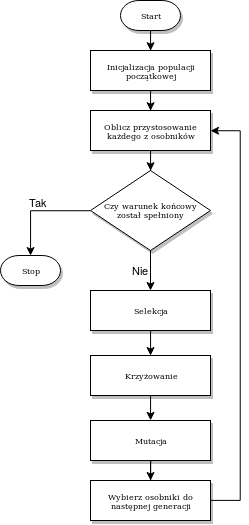
\includegraphics[width=0.4\textwidth]{img/alg_ewo_szkic.png}
    \caption{Ogólny schemat działania algorytmu ewolucyjnego}
    \label{alg_ewo_img}
\end{figure}

Projektowanie algorytmu ewolucyjnego możemy podzielić na kilka oddzielnych części, są to: 
\begin{itemize}
    \item Reprezentacja - określa sposób zakodowania rozwiązania w chromosomie. Wybór reprezentacji chromosomu jest bardzo ważnym etapem 
    projektowania algorytmu. Odpowiednia reprezentacja może w znacznym stopniu wpłynąć na szybkość i jakość rozwiązań znajdowanych przez 
    algorytm, ponieważ to ona w dużej mierze określa sposób w jaki przeszukiwana będzie przestrzeń rozwiązań zadania. 
    Jako reprezentacje bardzo często stosowane są wektory lub macierze genów, gdzie gen może być pojedynczą liczbą całkowitą lub rzeczywistą. 
    Oczywiście jako sposób reprezentacji rozwiązania możemy wybrać dowolną strukturę danych, należy jednak pamiętać, że zdefiniowane później 
    operacje mutacji i krzyżowania muszą być dostosowane do wybranej struktury.
    
    \item Funkcja oceny - określa stopień przystosowania danego osobnika. Bardzo często funkcja oceny jest równoważna funkcji celu, którą 
    nasz algorytm ma minimalizować/maksymalizować, nie jest to jednak regułą. 

    \item Operator krzyżowania - jest jednym z operatorów używanych do generowania kolejnego pokolenia w algorytmach ewolucyjnych. Z założenia 
    przyjmuje on jako argumenty dwa lub więcej rozwiązań(rodziców) i generuje na ich podstawie nowe(dzieci), które łączą w sobie cechy rodziców. 
    [TODO: przykład]

    \item Operator mutacji - jest drugim z operatorów używanych do generowania następnych pokoleń w algorytmach ewolucyjnych. Jego celem jest 
    poszerzene obszaru przeszukiwanych rozwiązań. Ten operator powinien wprowadzać minimalną zmianę w rozwiązaniu, co zapobiega zbyt szybkiej 
    zbieżności algorytmu i pozwala na wprowadzenie dodatkowej różnorodności w populacji. Należy pamiętać o tym, że wprowadzana zmiana nie może 
    być za duża, bo może to prowadzić do odwrotnego rezultatu, czyli zamiast różnicować rozwiązania nasz operator może je niszczyć.
    [TODO: przykład]

    \item Selekcja - określa sposób wyboru rodziców na których użyjemy operatora krzyżowania. Istnieje wiele opisanych metod selekcji\cite{SELECTION-METHODS} 
    takich jak np. metoda koła ruletki czy metoda rankingowa. Przy tworzeniu procedury selekcji należy pamiętać 
    o tym, że rozwiązania lepiej przystosowane powinny mieć większe szanse na zostanie rodzicami dla kolejnego pokolenia. Zapewnia to większe 
    szanse na wygenerowanie lepszych dzieci do następnej generacji.
    [TODO: przyklad]

    \item Wybór następnego pokolenia - ostateczny krok algorytmu, w którym wybieramy które osobniki wejdą w skład populacji początkowej w 
    kolejnej iteracji algorytmu. Podstawową składową tej populacji powinny być oczywiście osobniki wygenerowane za pomącą krzyżowania. Często 
    stosowaną praktyką jest również przepisywanie części najlepszych rozwiązań oraz kilku losowo wybranych z poprzedniego pokolenia. 

\end{itemize}
	\cleardoublepage

	\chapter{Ewolucyjne podejście do nieliniowego zadania transportowego}
\thispagestyle{chapterBeginStyle}

Tak jak powiedzieliśmy w poprzednim rozdziale, nieliniowe zadanie transportowe należy do zadań optymalizacyjnych, dla których trudno jest 
wyznaczyć dokładne rozwiązanie. Możemy za to za pomocą algorytmów przeszukujących zbiór dopuszczalnych rozwiązań, czyli algorytmów metaheurystycznych, 
postarać się wyznaczyć wystarczająco dobre rozwiązanie przybliżone. 

\section{Algorytmy metaheurystyczne}

Powiedzmy najpierw czym są algorytmy metaheurystyczne. Metaheurystyki są to algorytmy, które definiują sposób w jaki ma być przeszukiwany zbiór 
dopuszczalnych rozwiązań zdefiniowanego problemu. Znajdują one zastosowanie w przypadkach kiedy nie znamy algorytmów, które wyznaczają rozwiązanie 
dokładne lub ich koszt jest zbyt duży. Do tego typu problemów możemy zaliczyć rozważane tutaj nieliniowe zadanie transportowe. Minusem 
stosowania algorytmów metaheurystycznych jest fakt, że nie dają one gwarancji na znalezienie wystarczająco dobrego rozwiązania.

\subsection{Algorytmy ewolucyjne}
Algorytmy ewolucyjne stanowią podzbiór algorytmów metaheurystycznych. Sposób ich działania jest inspirowany przez zjawisko ewolucji występujące 
w naturze. Działają one na podzbiorach przestrzeni wszystkich rozwiązań, które nazywamy \textbf{populacjami}. Przy użyciu specjalnie zdefiniowanych 
operatorów, na podstawie jednej populacji tworzona jest kolejna zawierająca w sobie lepsze rozwiązania, nazywane dalej \textbf{chromosomami} 
lub \textbf{osobnikami}.

Na początku działania algorytmu generowana jest w sposób losowy populacja startowa. Procedurę generowania pojedynczego osobnika lub 
całej populacji nazywać będziemy \textbf{inicjalizacją}. Następnie na przestrzeni pokoleń (iteracji algorytmu) 
populacja ewoluuje generując coraz lepsze rozwiązania. W każdej iteracji pewna część osobników zostaje wybrana do reprodukcji. Procedurę wyboru 
rodziców do reprodukcji nazywać będziemy \textbf{selekcją}. Wybrane osobniki krzyżujemy między sobą, tworząc w ten sposób nowe, 
posiadające cechy wybranych wczesniej rodziców. Następnie losowo wybrane osobniki ulegają mutacji. 
Ostatecznie z otrzymanych osobników tworzona jest nowa populacja, która będzie stanowić bazę dla kolejnej iteracji algorytmu. Algorytm kończy 
działanie w momencie kiedy zostanie spełniony warunek końcowy, którym może być np. wygenerowanie wystarczająco dobrego rozwiązania lub 
przejście określonej liczby iteracji.

Ogólny schemat działania algorytmu ewolucyjnego przedstawiono w postaci pseudokodu \ref{alg_ewo} oraz schematu blokowego \ref{alg_ewo_img}.

\begin{pseudokod}[H]
\label{alg_ewo}
    \caption{Ogólny schemat działania algorytmu ewolucyjnego}
    $P_t$: Populacja w t-tej iteracji algorytmu\;
    $O_t$: Populacja dzieci w t-tej iteracji algorytmu\;
    \BlankLine
    $t \gets 0$\;
    inicjalizacja $P_t$\;
    \BlankLine
    \While{Warunek końcowy nie został spełniony} {
        $parents \gets$ selekcja z $P_t$\;
        $O_{t+1} \gets$ zastosuj operator krzyżowania na $parents$\;
        $O_{t+1} \gets$ zastosuj operator mutacji na $O_{t+1}$\;
        $P_{t+1} \gets$ wybierz osobniki do następnej generacji z $O_{t+1}$\;
        $t \gets t+1$\;
    }
    \Return{najlepszy osobnik z $P_t$}\;
\end{pseudokod}

\begin{figure}[H]
    \centering        
    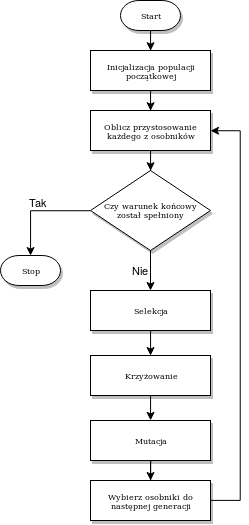
\includegraphics[width=0.6\textwidth]{img/alg_ewo_szkic.png}
    \caption{Ogólny schemat działania algorytmu ewolucyjnego.}
    \label{alg_ewo_img}
\end{figure}

Projektowanie algorytmu ewolucyjnego możemy podzielić na kilka oddzielnych części, są to: 
\begin{itemize}
    \item \textbf{Reprezentacja} - określa sposób zakodowania rozwiązania w chromosomie (osobniku). Wybór reprezentacji chromosomu jest bardzo ważnym etapem 
    projektowania algorytmu. Odpowiednia reprezentacja może w znacznym stopniu wpłynąć na szybkość i jakość rozwiązań znajdowanych przez 
    algorytm, ponieważ to ona w dużej mierze określa sposób w jaki przeszukiwana będzie przestrzeń rozwiązań zadania. 
    Jako reprezentacje bardzo często stosowane są wektory lub macierze genów, gdzie gen może być pojedynczą liczbą całkowitą lub rzeczywistą. 
    Oczywiście jako sposób reprezentacji rozwiązania możemy wybrać dowolną strukturę danych, należy jednak pamiętać, że zdefiniowane później 
    operacje mutacji i krzyżowania muszą być dostosowane do wybranej struktury.
    
    \item \textbf{Funkcja oceny} - określa stopień przystosowania danego osobnika. Bardzo często funkcja oceny jest równoważna funkcji celu, którą 
    nasz algorytm ma minimalizować/maksymalizować, nie jest to jednak regułą. 

    \item \textbf{Operator krzyżowania} - jest jednym z operatorów używanych do generowania kolejnego pokolenia w algorytmach ewolucyjnych. Z założenia 
    przyjmuje on jako argumenty dwa lub więcej rozwiązań (rodziców) i generuje na ich podstawie nowe (dzieci), które łączą w sobie cechy rodziców. 
    
    \begin{figure}[H]
        \centering        
        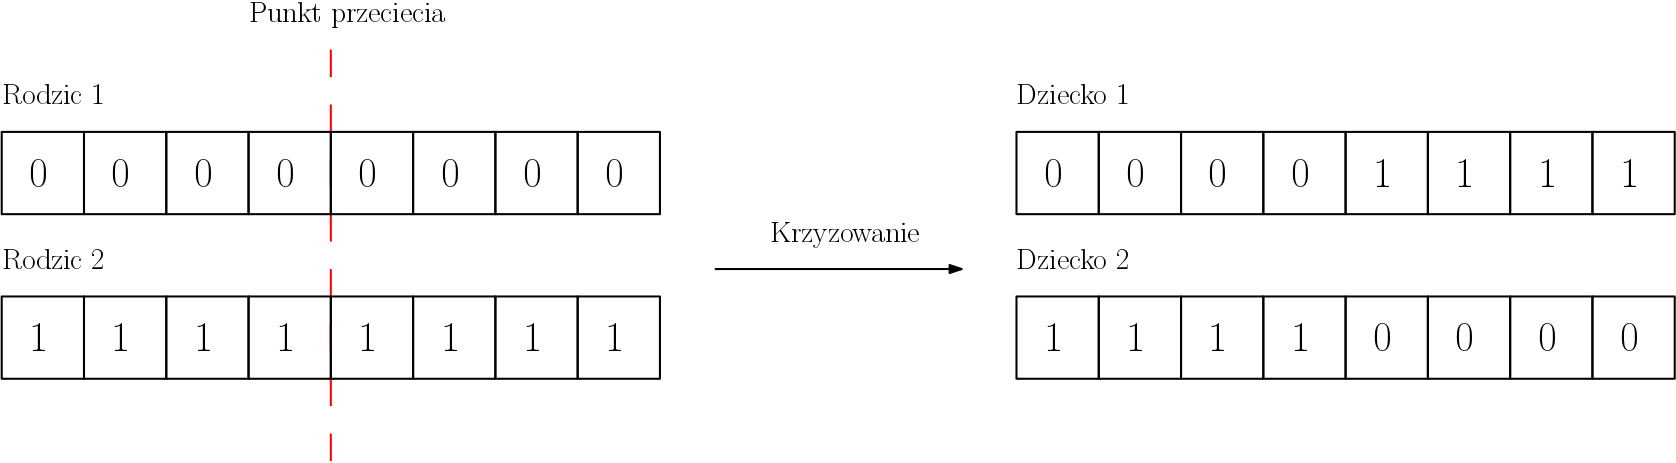
\includegraphics[width=0.9\textwidth]{img/cross_example.png}
        \caption{Przykład krzyżowania przez rozcięcie.}
    \end{figure}

    \item \textbf{Operator mutacji} - jest drugim z operatorów używanych do generowania następnych pokoleń w algorytmach ewolucyjnych. Jego celem jest 
    poszerzene obszaru przeszukiwanych rozwiązań. Ten operator powinien wprowadzać minimalną zmianę w rozwiązaniu, co zapobiega zbyt szybkiej 
    zbieżności algorytmu i pozwala na wprowadzenie dodatkowej różnorodności w populacji. Należy pamiętać o tym, że wprowadzana zmiana nie może 
    być za duża, bo może to prowadzić do odwrotnego rezultatu, czyli zamiast różnicować rozwiązania nasz operator może je niszczyć.
    
    \begin{figure}[H]
        \centering        
        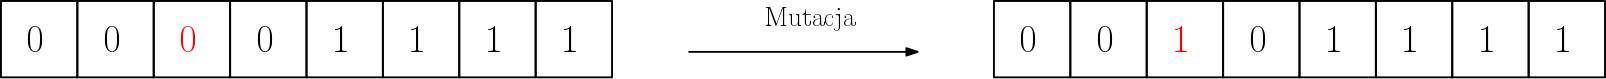
\includegraphics[width=0.9\textwidth]{img/mut_example.png}
        \caption{Przykład mutacji przez zanegowanie jednego bitu w rozwiązaniu.}
    \end{figure}

    \item \textbf{Selekcja} - określa sposób wyboru rodziców na których użyjemy operatora krzyżowania. Istnieje wiele opisanych metod selekcji\cite{SELECTION-METHODS} 
    takich jak np. metoda koła ruletki czy metoda rankingowa. Przy tworzeniu procedury selekcji należy pamiętać 
    o tym, że rozwiązania lepiej przystosowane powinny mieć większe szanse na zostanie rodzicami dla kolejnego pokolenia. Zapewnia to większe 
    szanse na wygenerowanie lepszych dzieci do następnej generacji.

    \item \textbf{Wybór następnego pokolenia} - ostateczny krok algorytmu, w którym wybieramy które osobniki wejdą w skład populacji początkowej w 
    kolejnej iteracji algorytmu. Podstawową składową tej populacji powinny być oczywiście osobniki wygenerowane za pomącą krzyżowania. Często 
    stosowaną praktyką jest również przepisywanie części najlepszych rozwiązań oraz kilku losowo wybranych z poprzedniego pokolenia. 

    \item \textbf{Parametry algorytmu} - do standardowych parametrów należą wielkość populacji, prawdopodobieństwo krzyżowania oraz prawdopodobieństwo 
    mutacji. Odpowiedni dobór parametrów ma kluczowe znaczenie dla efektywności oraz szybkości algorytmu.

\end{itemize}

W kolejnych sekcjach zaproponujemy algorytm ewolucyjny przystosowany do zadania transportowego, oparty na algorytmie zaprezentowanym przez 
dr. Zbigniewa Michalewicza\cite{ALG-GEN-BOOK}.


\section{Reprezentacja chromosomu}
W opisywanym algorytmie jako reprezentacje rozwiązania przyjęto macierz:
$$V = (v_{ij}) \text{, gdzie } 1 \le i \le length(supply) \land 1 \le j \le length(demand)$$

Rozwiązanie jest zakodowane w taki sposób, że komórka macierzy o indeksie $[i, j]$ określa ilość transportowanego towaru 
między $i$-tym punketm nadania i $j$-tym punktem odbioru. Jest to jedna z najbardziej naturalnych reprezentacji rozwiązania 
dla zadania transportowego.

\begin{table}[h!]
    \begin{center}
        \begin{tabular}{c||ccccc||c}
              & $s_1$ & $s_2$ & $s_3$ & $s_4$ & $s_5$ & $demand$ \\ 
            \hline
            \hline
            $d_1$ & 0.0 & 7.0 & 5.0 & 0.0 & 0.0 & 12.0 \\
            $d_2$ & 5.0 & 0.0 & 0.0 & 0.0 & 5.0 & 10.0 \\
            $d_3$ & 3.0 & 0.0 & 0.0 & 0.0 & 0.0 & 3.0 \\
            $d_4$ & 0.0 & 0.0 & 0.0 & 3.0 & 7.0 & 10.0 \\
            $d_5$ & 2.0 & 0.0 & 0.0 & 10.0 & 0.0 & 12.0 \\
            \hline
            \hline
            $supply$ & 10.0 & 7.0 & 5.0 & 13.0 & 12.0 & \\ 
        \end{tabular}
    \end{center}
    \caption{Przykładowe rozwiązanie.}
\end{table}

Aby ograniczenia zadania zostały zachowane, macierz rozwiązania musi spełniać następujące warunki:
$$\sum_{j=1}^{m} v_{ij} = supply[i], \text{ dla } i = 1, 2, \dots, n \text{, gdzie } n = length(supply)$$
$$\sum_{i=1}^{n} v_{ij} = demand[j], \text{ dla } j = 1, 2, \dots, m \text{, gdzie } m = length(demand)$$
$$v_{ij} \ge 0, \text{ dla } i = 1, 2, \dots, n \text{ i } j = 1, 2, \dots, m$$


\section{Inicjalizacja chromosomu}
Projektując procedurę inicjalizacji rozwiązania musimy pamiętać o tym, żeby generowane rozwiązania spełniały ograniczenia przedstawione 
w poprzedniej sekcji oraz obejmowały jak największą część przestrzeni wszystkich rozwiązań. Zaproponowana procedura przyjmuje jako argumenty 
wektory popytu i podaży. Iterując po kolejnych, losowych komórkach macierzy przypisujemy im wartość $val = \min(supply[i], demand[j])$, gdzie 
$i, j$ są indeksami wylosowanej komórki macierzy, a $supply[i]$ oraz $demand[j]$ odpowiadającymi im wartościami w wektorach popytu i podaży. 
Następnie zmniejszamy wartości w wektorach o wpisaną wartość $val$. W ten sposób ograniczenia zadania zostają spełnione. Wygenerowane rozwiązania są 
wierzchołkami sympleksu, opisującego wypukły brzeg przestrzeni dopuszczalnych rozwiązań.

\begin{pseudokod}[H]
    \label{inicjalizacja-1}
    \SetKwInOut{Input}{Wejście}
    \SetKwInOut{Output}{Wyjście}
    \caption{Procedura inicjalizacji chromosomu}
    \Input{$supply$ - wektor popytu rozmiaru $n$, $demand$ - wektor podaży rozmiaru $m$}
    \Output{$V$ - zainicjalizowana macierz}
    \BlankLine
    $V \gets zeros(n, m)$\tcc*[r]{generujemy macierz zerową rozmiaru $n \times m$}
    $indices \gets$ lista wszystkich indeksów macierzy $V$ w losowej kolejności\;
    \BlankLine
    \For{$(s, d) \in indices$} {
        $val \gets \min(demand[d], supply[s])$\;
        $demand[d] \gets demand[d] - val$\;
        $supply[s] \gets supply[s] - val$\;
        $V[s, d] \gets val$\;
    }

    \Return{$V$}
\end{pseudokod}

\begin{example}
    Przyklad inicjalizacji dla 3 dostawców i 2 odbiorców.

    1. Weźmy następujące wektory popytu i podaży:
    $$demand = [10, 12]$$
    $$supply = [8, 7, 7]$$

    2. Wygenerujmy zerową macierz rozwiązania $V$.

    $$
        V
        =
        \begin{bmatrix}
            0 & 0 & 0 \\
            0 & 0 & 0 \\
        \end{bmatrix}
    $$

    3. Wygenerujmy losowy wektor permutacji wszystkich indeksów macierzy rozwiązania.

    $$indices = [(1,1), (3,2), (1,2), (2,1), (3,1), (2,2)]$$

    4. Zainicjalizujmy komórki macierzy $V[s,d] = \min(supply[s], demand[d])$, gdzie $(s,d) \in indices$
    
    $$
        \begin{bmatrix}
            0 & 0 & 0 \\
            0 & 0 & 0 \\
        \end{bmatrix}
        \rightarrow^{(1,1)}
        \begin{bmatrix}
            \textbf{8} & 0 & 0 \\
            0 & 0 & 0 \\
        \end{bmatrix}
        \rightarrow^{(3,2)}
        \begin{bmatrix}
            8 & 0 & 0 \\
            0 & 0 & \textbf{7} \\
        \end{bmatrix}
        \rightarrow^{(1,2)}
        \begin{bmatrix}
            8 & 0 & 0 \\
            \textbf{0} & 0 & 7 \\
        \end{bmatrix}
        \rightarrow^{(2,1)}
        $$
        $$
        \begin{bmatrix}
            8 & \textbf{2} & 0 \\
            0 & 0 & 7 \\
        \end{bmatrix}
        \rightarrow^{(3,1)}
        \begin{bmatrix}
            8 & 2 & \textbf{0} \\
            0 & 0 & 7 \\
        \end{bmatrix}
        \rightarrow^{(2,2)}
        \begin{bmatrix}
            8 & 2 & 0 \\
            0 & \textbf{5} & 7 \\
        \end{bmatrix}
    $$

    5. W tym momencie kończymy procedurę inicjalizacji, nasza macierz rozwiązania ma postać:
    $$
    V
    =
    \begin{bmatrix}
        8 & 2 & 0 \\
        0 & 5 & 7 \\
    \end{bmatrix}
    $$
\end{example}


\section{Operator krzyżowania}
Operator krzyżowania został zdefiniowany jako kombinacja wypukła dwóch rodziców. W ten sposób w wyniku jednego krzyżowania powstają dwa nowe 
rozwiązania.

\begin{pseudokod}[H]
    \label{krzyżowanie}
    \SetKwInOut{Input}{Wejście}
    \SetKwInOut{Output}{Wyjście}
    \caption{Operator krzyżowania}
    \Input{$P_1, P_2$ - rodzice wybrani do krzyżowania}
    \Output{$O_1, O_2$ - otrzymane dzieci}
    \BlankLine
    $c_1 \gets rand(0,\dots,1)$\tcc*[r]{losujemy liczbę z przedziału $[0,1]$}
    $c_2 \gets 1.0 - c_1$\;
    $O_1 \gets c_1 * P_1 + c_2 * P_2$\;
    $O_2 \gets c_2 * P_1 + c_1 * P_2$\;
    \Return{$(O_1, O_2)$}\;
\end{pseudokod}

Zdefiniowany tak operator krzyżowania nie narusza ograniczeń zadania, ponieważ przestrzeń rozwiązań jest wypukła. Wynika z tego, że jeśli 
rodzice spełniali ograniczenia, to otrzymane w ten sposób dzieci również muszą spełniać ograniczenia.

\begin{example}
    Przykład zastowania operatora krzyżowania dla macierzy rozwiązania rozmiaru $3 \times 2$.

    1. Wybierzmy rodziców do krzyżowania:

    $$
        P_1
        =
        \begin{bmatrix}
            8 & 2 & 0 \\
            0 & 5 & 7 \\
        \end{bmatrix}
    $$
    $$
        P_2
        =
        \begin{bmatrix}
            0 & 3 & 7 \\
            8 & 4 & 0 \\
        \end{bmatrix}
    $$

    2. Wylosujmy współczynniki $c_1 = 0.6$ oraz $c_2 = 1 - c_1 = 0.4$

    3. Zastosujmy krzyżowanie.

    $$
        O_1
        =
        0.6
        \begin{bmatrix}
            8 & 2 & 0 \\
            0 & 5 & 7 \\
        \end{bmatrix}
        +
        0.4
        \begin{bmatrix}
            0 & 3 & 7 \\
            8 & 4 & 0 \\
        \end{bmatrix}
        =
        \begin{bmatrix}
            4.8 & 2.4 & 2.8 \\
            3.2 & 4.6 & 4.2 \\
        \end{bmatrix}
    $$
    $$
        O_2
        =
        0.4
        \begin{bmatrix}
            8 & 2 & 0 \\
            0 & 5 & 7 \\
        \end{bmatrix}
        +
        0.6
        \begin{bmatrix}
            0 & 3 & 7 \\
            8 & 4 & 0 \\
        \end{bmatrix}
        =
        \begin{bmatrix}
            3.2 & 2.6 & 4.2 \\
            4.8 & 4.4 & 2.8 \\
        \end{bmatrix}
    $$

\end{example}

\section{Operator mutacji}
Operator mutacji opiera się na modyfikacji rozwiązania poprzez wybranie z niego podmacierzy i jej ponowną inicjalizacje(patrz \ref{mutacja}). 
Załóżmy, że mamy $n$ punktów nadania i $m$ punktów odbioru. Wybierzmy jako kandydata do mutacji macierz $V = (v_{ij})$, gdzie $1 \le i \le n$ i 
$1 \le j \le m$. Podmacierz $W = w_{ij}$ jest tworzona w następujący sposób:

\begin{itemize}
    \item Losujemy podzbiór $k$ indeksów $\{i_1, \dots, i_k\}$ ze zbioru $\{1, \dots, n\}$ oraz podzbiór $l$ indeksów $\{j_1, \dots, j_l\}$ 
    ze zbioru $\{1, \dots, m\}$, $2 \le k \le n$ i $2 \le l \le m$.
    \item Tworzymy podmacierz $W$ składającą się z takich elementów macierzy $V$, które zostały wylosowane, tzn. element $v_{ij} \in V$ 
    zostaje włączony do podmacierzy $W$ tylko jeśli $i \in \{i_1, \dots, i_n\}$ oraz $j \in \{j_1, \dots, j_l\}$.
\end{itemize}

Dla stworzonej macierzy $W$ tworzymy nowe wektory $demand_W$ i $supply_W$ w następujący sposób:
$$supply_W[i] = \sum_{j \in \{j_1, \dots, j_l\}} v_{ij}, \text{ dla } 1 \le i \le k$$
$$demand_W[j] = \sum_{i \in \{i_1, \dots, i_k\}} v_{ij}, \text{ dla } 1 \le j \le l$$

Następnie na nowo inicjalizujemy podmacierz $W$ macierzy $V$ używając stworzonych wektorów $demand_W$ oraz $supply_W$ do określenia popytu i podaży 
w wybranych punktach nadania i odbioru. Po zakończeniu inicjalizacji przepisujemy wartości z podmacierzy $W$ z powrotem w odpowiadające miejsca 
macierzy $V$.

\begin{pseudokod}[H]
    \label{mutacja}
    \caption{Operator mutacji}
    \SetKwInOut{Input}{Wejście}
    \SetKwInOut{Output}{Wyjście}
    \Input{$V$ - osobnik wybrany do mutacji wielkości $n \times m$, $k, l$ - wielkość podmacierzy}
    \Output{$V$ - osobnik po mutacji}
    \BlankLine
    $supply\_idx \gets$ wylosuj podzbiór długości $k$ ze zbioru $\{1, \dots, n\}$\;
    $demand\_idx \gets$ wylosuj podzbiór długości $l$ ze zbioru $\{1, \dots, m\}$\;
    $W \gets zeros(k, l)$\tcc*[r]{generujemy macierz zerową rozmiaru $k \times l$}
    \BlankLine
    \For{$i \in \{1, \dots, k\}$} {
        \For{$j \in \{1, \dots, l\}$} {
            $W[i, j] \gets V[demand\_idx[j], supply\_idx[i]]$\;
        }
    }
    \BlankLine
    $supply\_vec \gets zeros(k)$\tcc*[r]{generujemy wektor zerowy długości k}
    $demand\_vec \gets zeros(l)$\tcc*[r]{generujemy wektor zerowy długości l}
    \BlankLine
    \For{$i \in supply\_idx$} {
        $supply\_vec[i] \gets \sum_{j \in demand\_idx} V[i, j]$\;
    }
    \BlankLine
    \For{$j \in demand\_idx$} {
        $demand\_vec[j] \gets \sum_{i \in supply\_idx} V[i, j]$\;
    }
    \BlankLine
    $W \gets inicjalizacja(W, demand\_vec, supply\_vec)$\;
    \BlankLine
    \For{$i \in \{1, \dots, k\}$} {
        \For{$j \in \{1, \dots, l\}$} {
            $V[demand\_idx[j], supply\_idx[i]] \gets W[i, j]$\;
        }
    }
    
    \Return{$V$}
\end{pseudokod}

Zdefiniowano dwa operatory mutacji. Różnią się one jedynie procedurą inicjalizacji. W pierwszym używamy tej samej procedury, którą inicjalizujemy 
nowe chromosomy podczas generowania populacji początkowej (patrz \ref{inicjalizacja-1}). Druga jest modyfikacją tej procedury. Modyfikacja polega na tym, że zamiast wybierać 
jako wartość pola $val = \min(demand[j], supply[i])$ wybieramy liczbę z zakresu $[0, val]$. Zmiana ta powoduje, że otrzymana macierz może naruszać 
ograniczenia zadania, dlatego po wstępnym wyznaczeniu wartości naprawiamy rozwiązanie poprzez zrobienie wymaganych dodawań w taki sposób, żeby 
rozwiązanie spełniało ograniczenia.

Poniżej przedstawiono schemat zmodyfikowanej procedury inicjalizacji w postaci pseudokodu.

\begin{pseudokod}[H]
    \label{inicjalizacja-2}
    \caption{Zmodyfikowana procedura inicjalizacji}
    \SetKwInOut{Input}{Wejście}
    \SetKwInOut{Output}{Wyjście}
    \Input{$supply$ - wektor podaży rozmiaru $n$, $demand$ - wektor popytu rozmiaru $m$}
    \Output{$V$ - zainicjalizowana macierz}
    \BlankLine
    $V \gets zeros(n, m)$\tcc*[r]{generujemy macierz zerową rozmiaru $n \times m$}
    $indices \gets$ lista wszystkich indeksów macierzy $V$ w losowej kolejności\;
    \BlankLine
    \For{$(s, d) \in indices$} {
        $val \gets$ wartość z przedziału $[0, \min(demand[d], supply[s])]$\;
        $demand[d] \gets demand[d] - val$\;
        $supply[s] \gets supply[s] - val$\;
        $V[s, d] \gets val$\;
    }
    \BlankLine
    \For{$(s, d) \in indices$} {
        $val \gets \min(demand[d], supply[s])$\;
        $demand[d] \gets demand[d] - val$\;
        $supply[s] \gets supply[s] - val$\;
        $V[s, d] \gets V[s, d] + val$\;
    }

    \Return{$V$}
\end{pseudokod}

\section{Funkcje oceny}
W przypadku omawianego problemu funkcja oceny jest równoważna odwrotności funkcji celu dla zadania transportowego. Powinna więc mieć postać:
$$\frac{1}{\sum_{i=1}^{n}\sum_{j=1}^{m} f(v_{ij})}$$
gdzie $f(v_{ij})$ jest dowolną funkcją przyjmującą jako argument ilość towaru transportowanego między punktami $i$ oraz $j$.
Bierzemy odwrotnośc, ponieważ chemy minimalizować funkcję celu, tzn. im mniejszy koszt osobnika, tym większa wartość funkcji przystosowania.

Przykładowe funkcje celu znajdują się w części eksperymentalnej.

\section{Metoda selekcji}
W algorytmie zastosowano standardową metodę selekcji - metodę koła ruletki. W tej metodzie lepiej przystosowane osobniki mają odpowiednio większe 
szanse na to, że zostaną wybrane do puli rodziców dla następnej generacji. Polega ona na tym, że dla każdego osobnika z populacji 
przyporzątkowujemy odpowiednio duży wycinek koła. Wielkość wycinka zależy od wartości funkcji przystosowania, jaką osiągnął dany chromosom. 
Następnie losujemy kołem tyle razy, ile rodziców chcemy otrzymać. Metoda ta pozwala na to, że jeden osobnik zostanie wybrany na rodzica kilkukrotnie.

Bardziej formalnie procedura została przedstawiona na poniższym pseudokodzie.

\begin{pseudokod}[H]
    \label{selekcja}
    \caption{Procedura selekcji}
    \SetKwInOut{Input}{Wejście}
    \SetKwInOut{Output}{Wyjście}
    \Input{$population$ - populacja chromosomów, $n$ - ilość rodziców do wybrania}
    \Output{$parents$ - wektor wybranych rodziców}
    \BlankLine
    $parents \gets$ stwórz pusty wektor długości n\;
    $k \gets length(population)$\;
    $wheel \gets zeros(k)$\tcc*[r]{Generujemy wektor zerowy długości $n$}
    \BlankLine
    $total \gets \sum_{i=1}^{k} population[i].cost$\;
    $wheel[1] \gets population[1].cost / total$\;
    \For{$i \in 2,\dots, k$} {
        $wheel[i] \gets population[i].cost / total + wheel[i-1]$\;
    }
    \BlankLine
    \For{$i \in 1,\dots, n$} {
        $num \gets rand(0,\dots, 1)$\tcc*[r]{losujemy wycinek koła}
        $selectedIdx \gets$ wybierz pierwszy taki $x$, że $wheel[x] \ge num$\;
        $parents[i] \gets population[selectedIdx]$\;
    }

    \Return{$parents$}
\end{pseudokod}

\begin{example}
    Przykład konstrukcji koła ruletki dla populacji 5 osobników. 

    Weźmy populację liczącą 5 osobników $V_1, \dots, V_5$. Niech wartość funkcji przystosowania dla osobnika $V_i$ będzie równa $c_i$.

    Załużmy, że $c_1 = 5, c_2 = 10, c_3 = 15, c_4 = 20, c_5 = 25$.

    1. Tworzymy zerowy wektor o długości równej wielkości populacji, czyli w naszym wypadku długości 5.

    $$wheel = [0, 0, 0, 0, 0]$$

    2. Sumujemy wartość funkcji przystosowania wszystkich osobników w populacji.

    $$total = \sum_{i=1}^{5} c_i = 75$$

    3. Obliczamy kolejne przedziały dla każdego z osobników.

    $$wheel[1] = c_1 / total = 0.0667$$
    $$wheel[2] = c_2 / total + wheel[1] = 0.1333 + 0.0667 = 0.2$$
    $$wheel[3] = c_3 / total + wheel[2] = 0.2 + 0.2 = 0.4$$
    $$wheel[4] = c_4 / total + wheel[3] = 0.2667 + 0.4 = 0.6667$$
    $$wheel[5] = c_5 / total + wheel[4] = 0.3333 + 0.6667 = 1$$

    4. Ostatecznie nasze koło ma postać $wheel = [0.0667, 0.2, 0.4, 0.6667, 1]$

    Teraz, aby wybrać rodzica losujemy liczbę z zakresu $[0, 1]$ i wybieramy osobnika, w którego przedziale znajduje się wylosowana liczba, np.
    załóżmy, że wylosowaliśmy liczbe $r = 0.5$. Szukamy wtedy w naszym wektorze $wheel$ takiej liczby $x \ge r$, która będzie najbliższa 
    naszemu $r$. W naszym przypadku jest to $0.6667$. Indeks wybranego rodzica jest indeksem na którym znajduje się $x$, czyli w tym wypadku $idx = 4$.
    Wybieramy więc jako rodzica osobnika $V_4$.

    Możemy łatwo zauważyć, że losując rodziców w ten sposób, osobniki z większą wartością funkcji przystosowania mają większe przedziały na kole 
    ruletki, a co za tym idzie mają wieksze szanse na to, że zostaną wybrane.
    
\end{example}

\section{Wersja równoległa}

Zaprojektowany w ten sposób algorytm możemy w dość łatwy sposób zrównoleglić. Przyjżyjmy się jeszcze raz jego strukturze. Bazą algorytmu jest 
populacja, która ewoluuje tworząc coraz lepsze, bardziej przystosowane rozwiązania. Zauważmy, że składa się ona z określonej liczby osobników, 
które są od siebie niezależne, to znaczy, że operacje wykonane na jednym osobniku populacji nie wpływają na inne osobniki. Przykładowo 
obliczając wartość funkcji przystosowania dla całej populacji nie musimy się martwić o kolejność w jakiej będziemy wybierać osobniki. Możemy więc 
podzielić populacje na mniejsze części i następnie zlecić obliczenie funkcji przystosowania poszczególnych części pojedynczym wątkom. W ten 
sposób, wszystkie części mogą być obliczane w tym samym czasie, co powinno skutkować skróceniem czasu całkowitych obliczeń dla całej populacji.

Podobnie możemy postąpić w przypadku zastosowania operatorów genetycznych, które również wpływają tylko na poszczególne osobniki, a nie na całą 
populację.

Kolejną opcją zrównoleglenia jest podział populacji na kilka mniejszych, które przez określoną liczbę pokoleń mogą ewoluować niezależnie 
od siebie. Dodatkowo dzięki temu, że częściowe populacje ewoluują niezależnie od siebie, mogą one przeszukiwać osobne części przestrzeni 
rozwiązań, co może pozytywnie wpłynąć na ostateczne rozwiązanie znalezione przez algorytm\cite{ISLAND-MODEL-PERFORMANCE}.


\subsection{Modele algorytmu}

Zaproponujmy i opiszmy dwa modele dla algorytmu:
\begin{itemize}
    \item Klasyczny
    \item Wyspowy
\end{itemize}

Na początku procedura inicjalizacji generuje losową populacje o określonej liczbie osobników i oblicza wartość funkcji oceny dla każdego z nich. 
Następnie przechodzimy do głównej pętli algorytmu, która kończy się w momencie kiedy populacja osiągnie maksymalną ilość generacji. 
Każdy z trybów różni się przebiegiem procedury \textit{nextGeneration} (patrz \ref{alg_main_img}), która tworzy nową generacje osobników.

\newpage

\begin{figure}[H]
    \centering        
    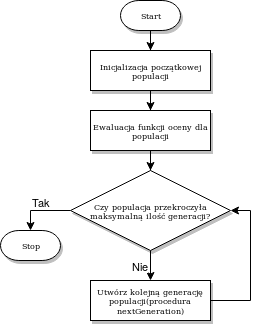
\includegraphics[width=0.6\textwidth]{img/alg_main.png}
    \caption{Przebieg zaimplementowanego algorytmu ewolucyjnego.}
    \label{alg_main_img}
\end{figure}

Model klasyczny nie różni się wiele od standardowego algorytmu ewolucyjnego. Mamy tutaj jedną populacje, która ewoluuje przez 
określoną przy starcie liczbę pokoleń. Wszystkie dostępne parametry algorytmu zostały krótko opisane w dalczej części pracy, 
w sekcji \textit{Parametry algorytmu}.

W modelu klasycznym zrównoleglenie odbywa się na poziomie pojedynczej iteracji (patrz \ref{next_gen_klasyczny_img}). 
Ewolucję populacji możemy podzielić tutaj na dwie części:
\begin{itemize}
    \item \textbf{Krzyżowanie} - w tej części między wątki rozdzielani są rodzice wybrani do krzyżowania. Następnie każdy z wątków generuje swoją część 
    dzieci oraz z określonym prawdopodobieństwem stostuje na nich operator mutacji i ostatecznie oblicza dla nich wartość funkcji oceny. 
    Dzieci są dodawane do kolejnej populacji.
    \item \textbf{Dopełnienie populacji} - w tej części do kolejnej populacji przepisywana jest część najlepszych rozwiązań oraz losowo wybranych osobników 
    z poprzedniej populacji. Następnie te dodane osobniki są poddawane mutacji i obliczana jest dla nich funkcja oceny.
\end{itemize}

\newpage

\begin{figure}[H]
    \centering        
    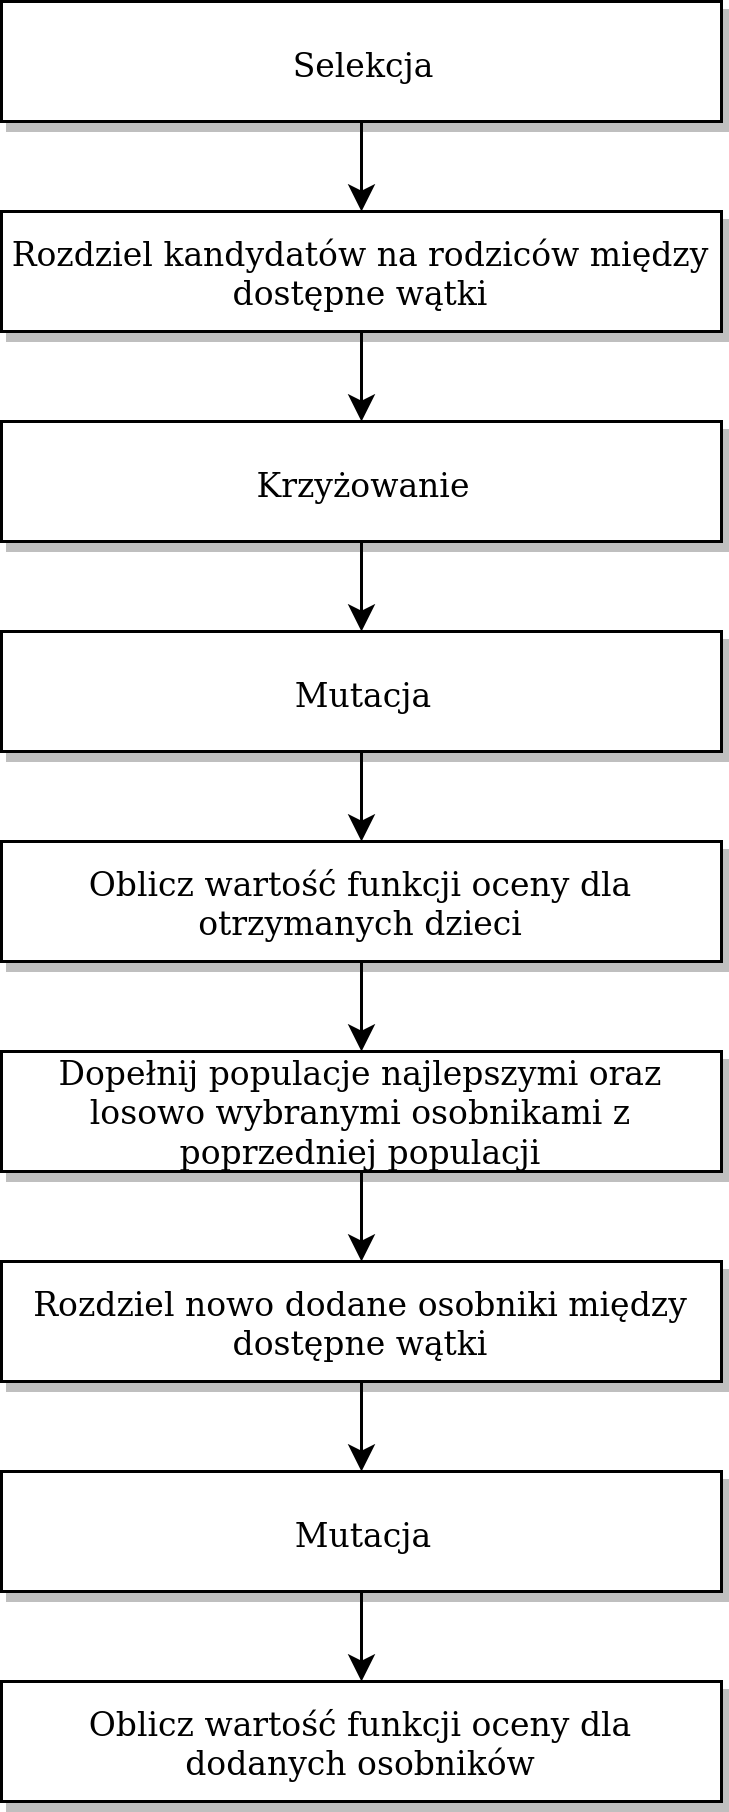
\includegraphics[width=0.4\textwidth]{img/next_gen_klasyczny.png}
    \caption{Przebieg procedury nextGeneration dla modelu klasycznego.}
    \label{next_gen_klasyczny_img}
\end{figure}

Model wyspowy różni się od klasycznego podejścia tym, że całkowita populacja jest tutaj rozdzielana na kilka mniejszych. Następnie każda z 
populacji częściowych ewoluuje niezależnie od innych przez określoną liczbę pokoleń. Po zakończeniu tego procesu wszystkie częściowe populacje 
są na nowo łączone w jedną. Następnie najlepsze rozwiązywanie jest zapisywane, a populacja zostaje na nowo podzielona na kilka mniejszych i 
cały proces się powtarza, do momentu w którym ilość generacji przekroczy określoną na początku liczbę. Na końcu najlepsze znalezione rozwiązanie 
jest zwracane.

W tym modelu zrównoleglenie obliczeń polega na tym, że przy każdym podziale populacji jeden wątek zarządza pojedynczą częścią populacji (patrz \ref{next_gen_wyspowy_img}).
Model ten skaluje się lepiej niż model klasyczny ze względu na to, że podzadania przydzielane wątkom są większe. Minusem jest tutaj to, że populacja 
musi być odpowiednio duża, żeby jej podział na mniejsze części się sprawdził.

\begin{figure}[H]
    \centering        
    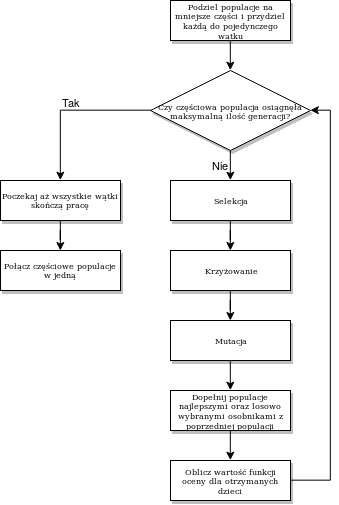
\includegraphics[width=0.7\textwidth]{img/next_gen_wyspowy.png}
    \caption{Przebieg procedury nextGeneration dla modelu wyspowego.}
    \label{next_gen_wyspowy_img}
\end{figure}

% W tym momencie każda z częściowych populacji w modelu wyspowym posiada takie same parametry. [...]

\section{Parametry algorytmu}
Opiszmy teraz krótko jakie parametry muszą zostać określone dla prezentowanego algorytmu i o czym będą one decydować.

\begin{itemize}
    \item $populationSize$ - rozmiar całkowitej populacji.
    \item $eliteProc$ - ułamek najlepszych rozwiązań, które zostają przepisane do następnego pokolenia.
    \item $mutationProb$ - prawdopodobieństwo z jaką występuje mutacja.
    \item $mutationRate$ - wielkość mutacji, określa stosunek rozmiaru podmacierzy, wybieranej do ponownej inicjalizacji podczas mutacji, 
    do macierzy rozwiązania.
    \item $crossoverProb$ - prawdopodobieństwo krzyżowania. Należy pamiętać o tym, że suma parametrów eliteProc i crossoverProb nie 
    może być większa niż $1$.
    \item $mode$ - tryb w jakim ma działać algorytm. Określa wybrany model ewolucji.
    \item $numberOfSeparateGenerations$ - określa ilość iteracji jakie wykona algorytm pomiędzy rozdzieleniem populacji na 
    mniejsze części, a ponownym jej scaleniem. Ma wpływ jedynie na model wyspowy. 
\end{itemize}

\section{Użyte technologie}
Do implementacji algorytmu zastosowano język Julia\cite{JULIA-PUB} w wersji 1.3. Julia jest stosunkowo nowym językiem programowania. Został zaprojektowany 
z myślą o zastosowaniach w obliczeniach numerycznych i analizie danych. Łączy on w sobie zalety języków niskopoziomowych i wysokopoziomowych takie jak szybkość 
i czytelność kodu. Testy pokazują, że program napisany w Julii może być równie szybki, jak odpowiadający mu program napisany w C\cite{JULIA-PERFORMANCE}. 
Dodatkową zaletą jest możliwość bezpośredniego wywoływania bibliotek napisanych w C, Fortranie i kilku innych językach popularnych w dziedzinie 
obliczeń numerycznych bezpośrednio z Julii.

Julia używa kompilatora JIT (just-in-time), który kompiluje program tuż przed jego wykonaniem, dzięki czemu jest szybsza 
niż języki interpretowane. Należy pamiętać o tym, że nie każdy program napisany w Julii będzie szybki. Wszystko zależy od jakości dostarczonego kodu.
Głównym czynnikiem, który wpływa na szybkość są typy. Julia jest językiem dynamicznie typowanym, jednak podczas kompilacji tworzone są warianty tej samej 
funkcji dla różnych typów (o ile to możliwe). Pozwala to pominąć kontrolę typów podczas wykonywania kodu i tym samym znacząco przyspieszyć jego działanie.
Dlatego pisząc kod w Julii powinniśmy pamiętać o tym, żeby unikać miejsc, w których kompilator będzie zmuszony do konwersji zmiennych do konkretnego typu. 
Aby identyfikować tego typu miejsca, możemy używać dostarczonych w bibliotece standardowej narzędzi, które pomagają analizować nasz kod. 
Warte wymienienia są tutaj:

\begin{itemize}
    \item pakiet $Profile$, który zbiera informacje o czasie wywołania kolejnych fragmentów kodu, dzięki czemu w łatwy sposób 
    możemy zidentyfikować fragmenty do dalszej optymalizacji. Pozwala on też śledzić liczbę ilość pamięci alokowanej przez konkretne fragmenty 
    kodu, co również w wielu przypadkach może okazać się przydatną informacją.
    \item makro $@code\_warntype$, które zwraca strukturę AST(abstract syntax tree) dla wykonywanego kodu, dzięki czemu możemy zobaczyć możliwe typy dla wszystkich zmiennych. 
    Dodatkowo miejsca w których kompilator nie jest w stanie jednoznacznie określić typu danej zmiennej jest zaznaczony na czerwono.
\end{itemize}

Julia udostępnia też środowisko uruchomieniowe $REPL$(read-eval-print loop), dzięki któremu możemy w bardzo łatwy sposób testować napisany kod. 
Dzięki dostępnym bibliotekom takim jak $Debugger.jl$ oraz $Rebugger.jl$ możemy w razie potrzeby debugować napisany kod z poziomu $REPL$ co 
znacznie przyspiesza znajdowanie błędów.

Ostatnie aktualizacje w znaczącym stopniu rozwinęły wsparcie języka dla obliczeń równoległych i rozproszonych. W tym momencie Julia oferuje wsparcie dla 
równoległości na poziomie wątków jak i procesów, co dodatkowo wpłynęło na wybór tego właśnie języka. Posiada własny protokół komunikacji między procesami, jednak 
istnieje również biblioteka implementująca najbardziej powszechny protokół MPI.

Biblioteka standardowa oferuje makra, które umożliwiają podział wszystkich iteracji pętli między wątki (makro $@threads$) lub procesy(makro $@distributed$). 
Taki podział zadań jest idealnym rozwiązaniem w przypadku kiedy iteracje pętli są niezależne od siebie i kolejność ich wykonywania nie ma 
znaczenia. Dokładnie taka sytuacja ma miejsce w implementowanym przez nas algorytmie, kiedy np. dzielimy populacje osobników na populacje 
częściowe, które ewoluują niezależnie od siebie. Dzięki temu mechanizm równoległości oferowany przez Julię idealnie sprawdza się w przedstawianym 
tutaj problemie.

	\cleardoublepage
	
	\chapter{Wyniki eksperymentalne}
\thispagestyle{chapterBeginStyle}
\label{rozdzial3}

W tym rozdziale pokazano wyniki testów dla prezentowanego programu oraz porównano go z innymi istniejącymi rozwiązaniami. 
Wszystkie eksperymenty zostały wykonane na serwerze Politechniki Wrocławskiej - \textit{OTRYT}. Serwer jest wyposażony w 4 procesory 
\textit{Intel(R) Xeon(R) CPU E7- 4850  @ 2.00GHz} posiadające po 10 rdzeni każdy oraz w 256 GB pamięci RAM. Serwer działa pod systemem 
\textit{Linux Debian} w wersji \textit{9.11}.

Dane testowe pochodzą częściowo z książki dr. Michalewicza(zadania $7 \times 7$ oraz $10 \times 10$)\cite{ALG-GEN-BOOK}, a częściowo 
zostały wygenerowane. Sposób generowania danych zaczerpnięto z publikacji \cite{GEN-TEST-DATA}. Dla wektorów popytu i podaży ustalano 
całkowity popyt/podaż, a następnie wypełniano je losowymi liczbami, zachowując przy tym warunek całkowitego popytu i podaży. 
Macierz kosztu generowano w taki sposób, że na początku ustalano dolne i górne ograniczenie wartości pojedynczego przewozu, a następnie 
macierz wypełniano losowymi liczbami z ustalonego zakresu. W przypadku jednej z funkcji kosztu, potrzebna była również macierz, która 
określa koszt stały, jaki ponosimy niezależnie od ilości towaru przewożonego między punktami. Macierz ta jest generowana w taki sam 
sposób, jak macierz kosztu. Charakterystyka poszczególnych zadań znajduje się w tabeli \ref{specyfika-zadan}.

\begin{table}[H]
    \begin{center}
        \begin{tabular}{c|c|c|c|c}
            Rozmiar & Popyt & Podaż & Zakres dla macierzy kosztu & Zakres dla macierzy kosztów stałych \\ 
            \hline
            $15 \times 15$ & $15000$ & $15000$ & $[3, 8]$ & $[50, 200]$ \\
            $30 \times 30$ & $3000$ & $3000$ & $[5, 15]$ & $[100, 400]$ \\
            $20 \times 70$ & $30000$ & $30000$ & $[3, 8]$ & $[200, 800]$ \\
            $30 \times 60$ & $25000$ & $25000$ & $[5, 15]$ & $[50, 100]$ \\
            $100 \times 100$ & $45000$ & $45000$ & $[3, 8]$ & $[100, 400]$ \\
        \end{tabular}
    \end{center}
    \caption{Charakterystyka wygenerowanych zadań.}
    \label{specyfika-zadan}
\end{table}


Funkcje kosztu użyte w testach w większości pochodzą z książki \cite{ALG-GEN-BOOK}. Przedstawiono je w tabeli \ref{funkcje-kosztu}. Dodatkowo 
użyto funkcji kosztu, która w przypadku przewozu towaru dodaje do kosztów liniowych koszt stały (Funkcja G w tabeli \ref{funkcje-kosztu}).

W eksperymentach porównano przedstawiany algorytm z wybranymi solverami wspieranymi przez system \textbf{GAMS}. Dostęp do solverów był możliwy poprzez serwis 
\textbf{NEOS Server} \cite{NEOS-1,NEOS-2,NEOS-3}, który pozwala na używanie kilkudziesięciu różnych solverów do optymalizacji problemów różnej kategorii. Do wybranych 
solverów należą:

\begin{itemize}
    \item LINDOGlobal
    \item CPLEX
    \item MINOS
    \item SNOPT
    \item scip
\end{itemize}

\newpage

\begin{table}[H]
    \begin{center}
        \begin{tabular}{ccl}
            Funkcja liniowa: & $f(x_{i,j})=$ & $c_{i,j} x_{i,j}$ \\
            \hline
            Funkcja A: & $f(x_{i,j})=$ & $c_{i,j}(\text{arctg}(1000 (x {i,j} - S))/\pi + 0.5 +$ \\
            & & $\text{arctg}(1000 (x {i,j} - 2 S))/\pi + 0.5 +$ \\
            & & $\text{arctg}(1000 (x {i,j} - 3 S))/\pi + 0.5 +$ \\
            & & $\text{arctg}(1000 (x {i,j} - 4 S))/\pi + 0.5 +$ \\
            & & $\text{arctg}(1000 (x {i,j} - 5 S))/\pi + 0.5)$ \\ 
            \hline
            Funkcja B: & $f(x_{i,j})=$ & $c_{i,j}[(x_{i,j}/5) (\text{arctg}(1000 x_{i,j})/\pi + 0.5) +$ \\
            & & $(1 - x_{i,j}/5) (\text{arctg}(1000(x_{i,j} - 5))/\pi + 0.5) +$ \\
            & & $(x_{i,j}/5 - 2) (\text{arctg}(1000(x_{i,j} - 10))/\pi + 0.5)]$ \\
            \hline
            Funkcja C: & $f(x_{i,j})=$ & $c_{i,j} x_{i,j}^2$ \\
            \hline
            Funkcja D: & $f(x_{i,j})=$ & $c_{i,j} \sqrt{x_{i,j}}$ \\
            \hline
            Funkcja E: & $f(x_{i,j})=$ & $c_{i,j}[(1 + (x_{i,j} - 10)^2)^{-1} +$ \\
            & & $(1 + (x_{i,j} - 11.25)^2)^{-1} +$ \\
            & & $(1 + (x_{i,j} - 8.75)^2)^{-1}]$ \\
            \hline
            Funkcja F: & $f(x_{i,j})=$ & $c_{i,j} x_{i,j} (\sin(5 \pi x_{i,j}/20) + 1)$ \\
            \hline
            Funkcja G: & $f(x_{i,j})=$ & $c_{i,j} x_{i,j} + c'_{i,j} y_{i,j}$ \\
        \end{tabular}
    \end{center}
    \caption{Funkcje kosztu}
    \label{funkcje-kosztu}
\end{table}

Z uwagi na to że serwis NEOS narzuca limit czasowy na wykonywanie pojedynczego zadania, przedstawione rozwiązania są najlepszym wynikiem znalezionym 
przez solver w czasie nie większym niż 8 godzin.

W następnych sekcjach zaprezentowano wyniki dla dwóch przedstawionych w poprzednim rozdziale modeli równoległości. Na początku zaprezentowano wyniki 
dla modelu klasycznego, który operuje na jednej populacji. Następnie z wynikami solverów zestawiono wyniki modelu wyspowego, w którym 
populacja jest dzielona na populacje częściowe. Na końcu porównano ze sobą oba modele.

Aby dostosować parametry dla testowanego systemu, na początku przeprowadzono serię testów dla różnych zadań i na podstawie tych wyników ustawiono 
odpowiednio parametry programu:

\begin{itemize}
    \item Rozmiar populacji: $100$(model klasyczny), $400$(model wyspowy)
    \item Prawdopodobieństwo krzyżowania: $0.5$
    \item Prawdopodobieństwo mutacji: $0.1$
    \item Wielkość mutacji: $0.05$
    \item Ułamek najlepszych osobników przepisywanych do nowej generacji: $0.2$
    \item Ilość niezależnych generacji dla populacji częściowej(model wyspowy): $50$
\end{itemize}

Maksymalną ilość iteracji algorytmu ustalono na $30000$.

\section{Model klasyczny algorytmu ewolucyjnego}

Wyniki przeprowazdone dla modelu klasycznego znajdują się w tabelach \ref{wyniki-0} oraz \ref{wyniki-1}. Tabela \ref{wyniki-0} zawiera porównanie 
modelu klasycznego z systemem GENOCOP (wyniki pochodzą z książki\cite{ALG-GEN-BOOK}), który pozwala optymalizować wszelkiego rodzaju zadania z ograniczeniami liniowymi i nieliniową funkcją celu. 
Widzimy tutaj, że nasz algorytm wypada lepiej niż system GENOCOP w większości testów. Udało się to osiągnąć dzięki zastosowaniu w algorytmie wiedzy o zadaniu
i dostosowaniu do niego reprezentacji rozwiązania oraz operatorów. Niestety nie udało się uzyskać wyników GENOCOPA dla zadania rozmiaru 
$10 \times 10$.

\newpage

\begin{table}[H]
    \begin{center}
        \resizebox{\textwidth}{!}{%
        \begin{tabular}{c|c|c|c|c|c|c}
            Rozmiar & Funkcja & \multicolumn{3}{c|}{Model klasyczny} & GENOCOP & LindoGlobal \\ \cline{3-5}
            zadania & celu & min & śr  & max &  & \\ 
            \hline
            \hline
            $7 \times 7$ & Liniowa & $1132.03$ & $1203.98$ & $1265.20$ & $---$ & $1132.0$ \\
            $7 \times 7$ & A & $0.0$ & $13.62$ & $67.0$ & $24.15$ & $4.26$ \\
            $7 \times 7$ & B & $180.65$ & $193.31$ & $224.07$ & $205.60$ & $183.59$ \\
            $7 \times 7$ & C & $2535.29$ & $2535.29$ & $2535.29$ & $2571.04$ & $2535.29$ \\
            $7 \times 7$ & D & $480.16$ & $565.57$ & $1046.45$ & $480.16$ & $480.16$ \\
            $7 \times 7$ & E & $204.71$ & $206.64$ & $221.52$ & $204.82$ & $204.84$ \\
            $7 \times 7$ & F & $67.31$ & $196.48$ & $351.38$ & $119.61$ & $70.25$ \\
            $7 \times 7$ & G & $1813.99$ & $1856.83$ & $1916.12$ & $---$ & $1796.0$ \\
            \hline
            $10 \times 10$ & Liniowa & $1179.0$ & $1188.96$ & $1213.24$ & $---$ & $1179.0$ \\
            $10 \times 10$ & A & $192.0$ & $200.2$ & $212.0$ & $---$ & $174.07$ \\
            $10 \times 10$ & B & $147.15$ & $154.19$ & $166.82$ & $---$ & $146.99$ \\
            $10 \times 10$ & C & $4401.65$ & $4401.65$ & $4401.65$ & $---$ & $4401.65$ \\
            $10 \times 10$ & D & $388.41$ & $409.36$ & $459.0$ & $---$ & $388.91$ \\
            $10 \times 10$ & E & $71.66$ & $72.99$ & $75.48$ & $---$ & $71.66$ \\
            $10 \times 10$ & F & $118.57$ & $215.90$ & $300.21$ & $---$ & $153.49$ \\
            $10 \times 10$ & G & $2010.50$ & $2075.15$ & $2194.69$ & $---$ & $1987.14$ \\
        \end{tabular}
        }
    \end{center}
    \caption{Wyniki dla zadań rozmiaru $7 \times 7$ i $10 \times 10$.}
    \label{wyniki-0}
\end{table}

Tabela \ref{wyniki-1} przedstawia wyniki dla pozostałych zadań wygenerowanych w sposób opisany na początku tego rozdziału. Porównano tutaj model klasyczny 
algorytmu ewolucyjnego z solverami MINOS oraz LINDOGlobal. O ile w przypadku MINOSa nie wiemy czy zwrócona wartość jest optimum globalnym, o tyle 
solver LINDOGlobal informuje o tym czy znalezione rozwiązanie to optimum lokalne czy globalne. Dodatkowo w przypadku optimum lokalnego, podaje on 
informację o najlepszym obliczonym dolnym ograniczeniu minimalizowanej funkcji. 

W przypadku jeśli LINDO zwrócił jedynie optimum lokalne przy wyniku znajduje się litera \textit{L}, w przypadku jeśli znaleziono optimum globalne, 
wynik jest oznaczony literą \textit{G}. W kolumnie \textit{luka} znaje się błąd względny między wartością otrzymaną a optimum globalnym, 
a więc $luka = \frac{|OPT - \tilde{C}|}{|OPT|} 100 \%$. W przypadku jeśli optimum globalne nie zostało znalezione, wiemy że w pesymistycznym 
przypadku znajduje się ono nie dalej niż ograniczenie dolne, tzn. $LB \le OPT$, gdzie $LB$ - ograniczenie dolne wyniku, oraz $OPT$ - optimum 
lokalne znalezione przez solver. W takim przypadku luka jest obliczana jako błąd względny między znalezionym rozwiązaniem, a dolnym ograniczeniem 
funkcji, czyli $luka = \frac{|LB - \tilde{C}|}{|LB|}$. 

Warto zwrócić uwagę na fakt, że podane dolne ograniczenie może być złej jakości, przez co błąd względny może wydawać się bardzo duży. Sytuacja 
taka miała miejsce w przypadku funkcji B oraz F, gdzie ograniczenie dolne dla wszystkich zestawów zadań testowych było równe $0$, czyli najmniejszemu 
możliwemu wynikowi w każdym zadaniu transportowym (z założenia wiemy, że koszt nie może być ujemny).

\newpage

\begin{table}[H]
    \begin{center}
        \resizebox{\textwidth}{!}{%
        \begin{tabular}{c|c||c|c|c|c||c||c|c||c|c}
            Rozmiar         & Funkcja      & \multicolumn{4}{c||}{Model klasyczny}               & MINOS         & \multicolumn{2}{c||}{LindoGlobal}& \multicolumn{2}{c}{CPLEX} \\ \cline{3-6} \cline{8-9} \cline{10-11}
            zadania         & celu         & min & śr  & max & luka                             &               & wynik & luka                    & wynik & luka \\
            \hline  
            \hline  
            $15 \times 15$ & Liniowa       & $54533.80$ & $55062.96$ & $55419.21$ & $1.24$      & $53862.32$    & $53862.32$ G & $0.00$           & $53862.32$ G & $0.00$ \\
            $15 \times 15$ & A             & $621.52$ & $627.98$ & $679.35$ & $40.42$           & $743.05$      & $470.50$ L & $21.27$            & $-$ & $-$ \\
            $15 \times 15$ & B             & $10607.71$ & $10657.78$ & $10933.70$ & $-$(*)      & $10581.32$    & $10454.80$ L & $-$(*)           & $-$ & $-$ \\
            $15 \times 15$ & C             & $5225274.22$ & $5225274.24$ & $5225274.30$ & $0.00$& $5225274.19$  & $5225274.19$ G & $0.00$         & $-$ & $-$ \\
            $15 \times 15$ & D             & $2187.99$ & $2211.11$ & $2273.07$ & $-$(*)         & $3229.68$     & $2314.41$ L & $-$(*)            & $-$ & $-$ \\
            $15 \times 15$ & E             & $1.20$ & $1.20$ & $1.20$ & $-$(*)                  & $33.13$       & $1.90$ L & $-$(*)               & $-$ & $-$ \\
            $15 \times 15$ & F             & $179.61$ & $180.16$ & $185.35$ & $-$(*)            & $11852.89$    & $59.23$ L & $-$(*)              & $-$ & $-$ \\
            $15 \times 15$ & G             & $62185.11$ & $62438.42$ & $63610.24$ & $9.65$      & $57366.75$    & $58546.32$ L & $2.74$           & $56985.03$ G & $0.00$ \\
            \hline  
            $30 \times 30$ & Liniowa       & $17365.25$ & $17479.06$ & $17795.71$ & $4.69$      & $16586.20$    & $16586.20$ G & $0.00$           & $16586.20$ G & $0.00$ \\
            $30 \times 30$ & A             & $1763.86$ & $1795.62$ & $1846.44$ & $27.60$        & $2260.7914$   & $2040.23$ L & $36.27$           & $-$ & $-$ \\
            $30 \times 30$ & B             & $2309.83$ & $2323.66$ & $2370.13$ & $-$(*)         & $2699.25$     & $2696.38$ L & $-$(*)            & $-$ & $-$ \\
            $30 \times 30$ & C             & $104650.12$ & $104650.40$ & $104651.73$ & $0.00$   & $104650.12$   & $104650.12$ G & $0.00$          & $-$ & $-$ \\
            $30 \times 30$ & D             & $2872.53$ & $2986.45$ & $3084.81$ & $-$(*)         & $3805.08$     & $2770.29$ L & $-$(*)            & $-$ & $-$ \\
            $30 \times 30$ & E             & $249.70$ & $249.84$ & $256.32$ & $61.33$           & $262.08$      & $285.34$ L & $66.14$            & $-$ & $-$ \\
            $30 \times 30$ & F             & $737.98$ & $823.82$ & $1063.14$ & $-$(*)           & $4630.83$     & $384.87$ L & $-$(*)             & $-$ & $-$ \\
            $30 \times 30$ & G             & $23533.16$ & $24813.93$ & $26622.49$ & $27.43$     & $19912.58$    & $20117.31$ L & $3.25$           & $19482.41$ G & $0.00$ \\
            \hline  
            $20 \times 70$ & Liniowa       & $102681.39$ & $102980.75$ & $103318.46$ & $4.57$   & $98476.50$    & $98476.50$ G & $0.00$           & $98476.50$ G & $0.00$ \\
            $20 \times 70$ & A             & $1926.42$ & $1997.94$ & $2099.43$ & $50.56$        & $2437.58$     & $1473.70$ L & $32.98$           & $-$ & $-$ \\
            $20 \times 70$ & B             & $19294.37$ & $19777.36$ & $20164.15$ & $-$(*)      & $19164.16$    & $18524.19$ L & $-$(*)           & $-$ & $-$ \\
            $20 \times 70$ & C             & $3356726.47$ & $3356779.29$ & $3356994.88$ & $0.00$& $3356719.33$  & $3356719.33$ G & $0.00$         & $-$ & $-$ \\
            $20 \times 70$ & D             & $6703.65$ & $6747.31$ & $6823.62$ & $-$(*)         & $8947.35$     & $6245.85$ L & $-$(*)            & $-$ & $-$ \\
            $20 \times 70$ & E             & $111.69$ & $113.03$ & $114.37$ & $-$(*)            & $221.51$      & $139.55$ L & $-$(*)             & $-$ & $-$ \\
            $20 \times 70$ & F             & $1594.30$ & $1644.51$ & $1697.70$ & $-$(*)         & $40503.51$    & $575.38$ L & $-$(*)             & $-$ & $-$ \\
            $20 \times 70$ & G             & $169931.77$ & $172399.15$ & $179244.49$ & $30.61$  & $135150.04$   & $134327.33$ L & $1.81$          & $131938.45$ G & $0.00$ \\
            \hline  
            $30 \times 60$ & Liniowa       & $145468.29$ & $146323.93$ & $146948.53$ & $7.67$   & $135028.71$   & $135028.71$ G & $0.00$          & $135028.71$ G & $0.00$ \\
            $30 \times 60$ & A             & $3532.37$ & $3544.40$ & $3631.18$ & $53.30$        & $4310.14$     & $2336.59$ L & $29.17$           & $-$ & $-$ \\
            $30 \times 60$ & B             & $26033.88$ & $26962.21$ & $27024.11$ & $-$(*)      & $26082.37$    & $26775.34$ L & $-$(*)           & $-$ & $-$ \\
            $30 \times 60$ & C             & $3283244.35$ & $3283249.33$ & $3283363.39$ & $0.00$& $3282784.56$  & $3282784.56$ G & $0.00$         & $-$ & $-$ \\
            $30 \times 60$ & D             & $11090.32$ & $11172.53$ & $11275.56$ & $-$(*)      & $13799.71$    & $Time out$ & $-$(*)             & $-$ & $-$ \\
            $30 \times 60$ & E             & $351.38$ & $351.57$ & $351.74$ & $-$(*)            & $526.34$      & $438.39$ L & $-$(*)             & $-$ & $-$ \\
            $30 \times 60$ & F             & $2981.06$ & $3498.70$ & $4404.37$ & $-$(*)         & $73724.43$    & $2390.12$ L & $-$(*)            & $-$ & $-$ \\
            $30 \times 60$ & G             & $176947.28$ & $180834.11$ & $187061.33$ & $27.54$  & $143907.24$   & $145316.08$ L & $2.51$          & $141761.66$ G & $0.00$ \\
            \hline  
            $100 \times 100$ & Liniowa     & $152120.75$ & $157299.10$ & $163931.16$ & $-$      & $138605.09$   & $Err$ & $-$                     & $138605.09$ G & $0.00$ \\
            $100 \times 100$ & A           & $4162.49$ & $4176.67$ & $4180.39$ & $-$            & $Err$         & $Err$ & $-$                     & $-$ & $-$ \\
            $100 \times 100$ & B           & $27175.45$ & $27320.57$ & $27993.08$ & $-$         & $Err$         & $Err$ & $-$                     & $-$ & $-$ \\
            $100 \times 100$ & C           & $1079937.33$ & $1080471.39$ & $1081882.67$ & $-$   & $Err$         & $Err$ & $-$                     & $-$ & $-$ \\
            $100 \times 100$ & D           & $12308.57$ & $12414.59$ & $12991.94$ & $-$         & $Err$         & $Err$ & $-$                     & $-$ & $-$ \\
            $100 \times 100$ & E           & $1531.03$ & $1531.32$ & $1532.51$ & $-$            & $Err$         & $Err$ & $-$                     & $-$ & $-$ \\
            $100 \times 100$ & F           & $---$ & $7405.57$ & $---$ &                        & $Err$         & $Err$ & $-$                     & $-$ & $-$ \\
            $100 \times 100$ & G           & $232139.70$ & $235821.75$ & $239278.53$ & $37.20$  & $175472.60$   & $Err$ & $-$                     & $171871.92$ G & $0.00$ \\
        \end{tabular}
        } 
    \end{center}
    \caption{Wyniki. (*) oznacza, że znalezione ograniczenie dolne dla problemu było słabej jakości, tzn. że było równe, lub bardzo bliskie $0$. 
        Wynik \textit{Timeout} oznacza, że solver nie znalazł rozwiązania w czasie 8 godzin. 
        Wynik \textit{Err} oznacza, że model był za duży dla solvera.}
    \label{wyniki-1}
\end{table}


Jak możemy zauważyć na prezentowanym porównaniu (tabela \ref{wyniki-1}) model klasyczny wypada lepiej niż solver MINOS w niemalże każdym teście. Jedyny 
wyjątek stanowi przypadek liniowej funkcji kosztu, gdzie MINOS zawsze znajdował optimum globalne. W przypadku funkcji B MINOS wypadał nieznacznie 
lepiej niż średni wynik dla modelu klasycznego, jednak była to z reguły różnica pomijalna (poniżej $1\%$). Z kolei dla funkcji D oraz F model 
klasyczny był znacznie lepszy niż MINOS, który w niektórych przypadkach zwrócił nawet kilkukrotnie gorszy wynik (funkcja F). Pozostałe wyniki były raczej 
zbliżone. Dla funkcji nieliniowych A-G i macierzy $100 \times 100$ MINOS nie zwrócił żadnego wyniku, ze względu na ograniczone zasoby pamięci oferowane 
przez serwis NEOS. 

Dla solvera LINDOGlobal, w wielu przypadkach wynikiem obliczeń było jedynie optimum lokalne (funkcje A,B,D,E,F). W tych przypadkach możemy 
porównywać odległości od dolnego ograniczenia wyniku wskazanego przez LINDOGlobal. Jest ono jednak w wielu przypadkach bardzo nieprecyzyjne. 
Mimo wszystko dla większości testów model klasyczny dawał wyniki zbliżone do wynkiów solvera. Przypadki łatwe, w których zostało znalezione optimum 
globalne były rozwiązywane przez model klasyczny z akceptowalnym błędem rzędu kilku procent.

Możemy zauważyć, że w przypadku liniowej funkcji kosztu model klasyczny radzi sobie gorzej niż pozostałe programy, jest to jednak problem bardzo 
łatwy i znamy dużo lepsze algorytmy, któwe są w stanie w krótkim czasie znaleźć dla niego optimum globalne. W tego typu prostych zadaniach stosowanie 
algorytmów metaheurystycznych, do których zalicza się opisywany algorytm ewolucyjny raczej mija się z celem. Stosunkowo słabe wyniki w tym przypadku 
są wynikiem tego, że otrzymywane osobniki nie są wystarczająco zróżnicowane. Z kolei dla dużo trudniejszych, nieliniowych 
funkcji celu, model klasyczny radzi sobie znacznie lepiej. Przede wszystkim prezentuje się dużo lepiej niż pozostałe solvery w porównaniu czasu 
potrzebnego na znalezienie rozwiązania. Dla algorytmu ewolucyjnego nawet problem rozmiaru $100 \times 100$ nie był żadną trudnością i 
był rozwiązywany w czasie kilkudziesięciu sekund. Pokazuje to główną zaletę algorytmów ewolucyjnych, jaką jest czas znajdowania rozwiązania.

Z uwagi na to, że w wielu przypadkach LINDO nie znalazł optimum globalnego, a ograniczenie dolne było niezadowalającej jakości, zdecydowano się 
porównać wyniki algorytmu ewolucyjnego z wynikami innych solverów, które również są w stanie optymalizować nieliniową funkcję celu 
przy liniowych ograniczeniach. Porównanie to znajduje się w tabeli \ref{wyniki-2}. Dla zwiększenia czytelności w tabeli pokazano jedynie średni wynik 
zwracany przez algorytm ewolucyjny. W kolumnach oznaczonych jako \% pokazano błąd względny pomiędzy najlepszym wynikiem dla konkretnego testu oraz 
wynikiem solvera. Takie porównanie daje lepszy obraz tego, jak prezentowany algorytm ewolucyjny wypada na tle innych istniejących rozwiązań.

\begin{table}[H]
    \begin{center}
        \resizebox{\textwidth}{!}{%
        \begin{tabular}{c|c||c|c||c|c||c|c||c|c||c|c}
            Rozmiar         & Funkcja    & \multicolumn{2}{c||}{Model klasyczny}  & \multicolumn{2}{c||}{MINOS} & \multicolumn{2}{c||}{scip} & \multicolumn{2}{c||}{SNOPT}& \multicolumn{2}{c}{LindoGlobal} \\ \cline{3-4} \cline{5-6} \cline{7-8} \cline{9-10} \cline{11-12}
            zadania         & celu       & śr. wynik & \%                        & wynik & \%                 & wynik & \%                & wynik & \%                & wynik & \% \\
            \hline
            \hline
            $15 \times 15$ & Liniowa     & $55062.96$ & $2.2$                    & $53862.32$ & \textbf{0.0}         & $53862.32$ & \textbf{0.0}        & $53862.32$ & \textbf{0.00}       & $53862.32$ & \textbf{0.0} \\
            $15 \times 15$ & A           & $627.98$ & $33.4$                     & $743.05$ & $57.9$          & $696.75$ & $48.1$         & $743.05$ & $57.9$         & $470.50$ & \textbf{0.0} \\
            $15 \times 15$ & B           & $10657.78$ & $1.9$                    & $10581.32$ & $1.2$         & $10630.82$ & $1.7$        & $10510.23$ & $0.5$        & $10454.80$ & \textbf{0.0} \\
            $15 \times 15$ & C           & $5225274.24$ & \textbf{0.0}                  & $5225274.19$ & \textbf{0.0}       & $5225274.19$ & \textbf{0.0}      & $5225274.19$ & \textbf{0.0}      & $5225274.19$ & \textbf{0.0} \\
            $15 \times 15$ & D           & $2211.11$ & \textbf{0.0}                     & $3229.68$ & $46.1$         & $2867.07$ & $29.7$        & $3229.68$ & $46.1$        & $2314.41$ & $4.67$ \\
            $15 \times 15$ & E           & $1.20$ & \textbf{0.0}                        & $33.13$ & $2660.8$         & $20.41$ & $1600.8$        & $33.50$ & $2691.7$        & $1.90$ & $58.3$ \\
            $15 \times 15$ & F           & $180.16$ & $204.2$                    & $11852.89$ & $19911.6$     & $2646.60$ & $4368.3$      & $10150.31$ & $17037.1$    & $59.23$ & \textbf{0.0} \\
            $15 \times 15$ & G           & $62438.42$ & $8.9$                    & $57366.75$ & \textbf{0.0}         & $57327.80$ & \textbf{0.0}        & $57366.75$ & \textbf{0.0}        & $58546.32$ & $2.1$ \\
            \hline
            $30 \times 30$ & Liniowa     & $17479.06$ & $5.4$                    & $16586.20$ & \textbf{0.0}         & $16586.20$ & \textbf{0.0}        & $16586.20$ & \textbf{0.0}        & $16586.20$ & \textbf{0.0} \\
            $30 \times 30$ & A           & $1795.62$ & \textbf{0.0}                     & $2260.7914$ & $25.9$       & $1888.26$ & $5.15$        & $2295.27$ & $27.8$        & $2040.23$ & $13.6$ \\
            $30 \times 30$ & B           & $2323.66$ & \textbf{0.0}                     & $2699.25$ & $16.2$         & $2664.35$ & $14.7$        & $2547.94$ & $9.7$         & $2696.38$ & $16.0$ \\
            $30 \times 30$ & C           & $104650.40$ & \textbf{0.0}                   & $104650.12$ & \textbf{0.0}        & $104650.12$ & \textbf{0.0}       & $144947.97$ & $38.5$      & $104650.12$ & \textbf{0.0} \\
            $30 \times 30$ & D           & $2986.45$ & $7.8$                     & $3805.08$ & $37.3$         & $3410.94$ & $23.1$        & $3805.08$ & $37.3$        & $2770.29$ & \textbf{0.0} \\
            $30 \times 30$ & E           & $249.84$ & \textbf{0.0}                      & $262.08$ & $4.9$           & $309.33$ & $23.8$         & $262.08$ & $4.9$          & $285.34$ & $14.2$ \\
            $30 \times 30$ & F           & $823.82$ & $114.0$                    & $4630.83$ & $1103.2$       & $957.32$ & $148.7$        & $4171.94$ & $984.0$       & $384.87$ & \textbf{0.0} \\
            $30 \times 30$ & G           & $24813.93$ & $24.6$                   & $19912.58$ & \textbf{0.0}         & $19981.01$ & $0.4$        & $19912.58$ & \textbf{0.0}        & $20117.31$ & $1.0$ \\
            \hline
            $20 \times 70$ & Liniowa     & $102980.75$ & $4.6$                   & $98476.50$ & \textbf{0.0}         & $98476.50$ & \textbf{0.0}        & $98476.50$ & \textbf{0.0}        & $98476.50$ & \textbf{0.0} \\
            $20 \times 70$ & A           & $1997.94$ & $35.5$                    & $2437.58$ & $65.4$         & $1781.99$ & $20.9$        & $2437.58$ & $65.4$        & $1473.70$ & \textbf{0.0} \\
            $20 \times 70$ & B           & $19777.36$ & $7.26$                   & $19164.16$ & $3.9$         & $18763.24$ & $1.8$        & $18438.52$ & \textbf{0.0}        & $18524.19$ & $0.5$ \\
            $20 \times 70$ & C           & $3356779.29$ & \textbf{0.0}                  & $3356719.33$ & \textbf{0.0}       & $3356719.33$ & \textbf{0.0}      & $7808433.26$ & $132.6$    & $3356719.33$ & \textbf{0.0} \\
            $20 \times 70$ & D           & $6747.31$ & $11.6$                    & $8947.35$ & $47.9$         & $6047.94$ & \textbf{0.0}         & $8947.35$ & $47.9$        & $6245.85$ & $3.27$ \\
            $20 \times 70$ & E           & $113.03$ & \textbf{0.0}                      & $221.51$ & $96.0$          & $176.21$ & $56.0$         & $221.51$ & $96.0$         & $139.55$ & $23.5$ \\
            $20 \times 70$ & F           & $1644.51$ & $186.0$                   & $40503.51$ & $6939.4$      & $7462.94$ & $1197.0$      & $40939.03$ & $7015.1$     & $575.38$ & \textbf{0.0} \\
            $20 \times 70$ & G           & $172399.15$ & $28.3$                  & $135150.04$ & $0.6$        & $135150.0$ & $0.6$        & $135150.0$ & $0.6$        & $134327.33$ & \textbf{0.0} \\
            \hline
            $30 \times 60$ & Liniowa     & $146323.93$ & $8.3$                   & $135028.71$ & \textbf{0.0}        & $135028.71$ & \textbf{0.0}       & $135028.71$ & \textbf{0.0}       & $135028.71$ & \textbf{0.0} \\
            $30 \times 60$ & A           & $3544.40$ & $51.7$                    & $4310.14$ & $84.5$         & $3767.46$ & $61.2$        & $4310.14$ & $84.5$        & $2336.59$ & \textbf{0.0} \\
            $30 \times 60$ & B           & $26962.21$ & $7.3$                    & $26082.37$ & $3.8$         & $26355.05$ & $4.9$        & $25126.84$ & \textbf{0.0}        & $26775.34$ & $6.6$ \\
            $30 \times 60$ & C           & $3283249.33$ & \textbf{0.0}                  & $3282784.56$ & \textbf{0.0}       & $3282784.56$ & \textbf{0.0}      & $9640058.72$ & $193.7$    & $3282784.56$ & \textbf{0.0} \\
            $30 \times 60$ & D           & $11172.53$ & $0.8$                    & $13799.71$ & $24.5$        & $11081.48$ & \textbf{0.0}        & $13799.71$ & $24.5$       & $Time out$ & $-$ \\
            $30 \times 60$ & E           & $351.57$ & \textbf{0.0}                      & $526.34$ & $49.7$          & $1158.46$ & $230.0$       & $526.34$ & $49.7$         & $438.39$ & $24.7$ \\
            $30 \times 60$ & F           & $3498.70$ & $46.4$                    & $73724.43$ & $2984.5$      & $6935.45$ & $190.2$       & $68411.66$ & $2762.3$     & $2390.12$ & \textbf{0.0} \\
            $30 \times 60$ & G           & $180834.11$ & $25.6$                  & $143907.24$ & \textbf{0.0}        & $143953.62$ & $0.1$       & $143907.24$ & \textbf{0.0}        & $145316.08$ & $0.9$ \\
            \hline
            $100 \times 100$ & Liniowa   & $157299.10$ & $13.5$                  & $138605.09$ & \textbf{0.0}        & $138605.09$ & \textbf{0.0}       & $138605.09$ & \textbf{0.0}       & $Err$ & $-$ \\
            $100 \times 100$ & A         & $4176.67$ & \textbf{0.0}                     & $Err$ & $-$                & $4657.38$ & $11.5$        & $25858.31$ & $519.1$      & $Err$ & $-$ \\
            $100 \times 100$ & B         & $27320.57$ & \textbf{0.0}                    & $Err$ & $-$                & $35556.19$ & $30.1$       & $35556.19$ & $30.1$       & $Err$ & $-$ \\
            $100 \times 100$ & C         & $1080471.39$ & $1.3$                  & $Err$ & $-$                & $1066457.36$ & \textbf{0.0}      & $15080858.45$ & $1314.1$  & $Err$ & $-$ \\
            $100 \times 100$ & D         & $12414.59$ & \textbf{0.0}                    & $Err$ & $-$                & $13910.55$ & $12.1$       & $15844.99$ & $27.6$       & $Err$ & $-$ \\
            $100 \times 100$ & E         & $1531.32$ & \textbf{0.0}                     & $Err$ & $-$                & $1741.40$ & $13.7$        & $1657.65$ & $8.2$         & $Err$ & $-$ \\
            $100 \times 100$ & F         & $7405.57$ & \textbf{0.0}                     & $Err$ & $-$                & $10064.85$ & $36.0$       & $31191.89$ & $321.2$      & $Err$ & $-$ \\
            $100 \times 100$ & G         & $235821.75$ & $34.3$                  & $175472.60$ & \textbf{0.0}        & $175517.69$ & \textbf{0.0}       & $175472.60$ & \textbf{0.0}       & $Err$ & $-$ \\
        \end{tabular}
        }
    \end{center}
    \caption{Porównanie modelu klasycznego algorytmu ewolucyjnego i innych dostępnych solverów.}
    \label{wyniki-2}
\end{table}

Jakość rozwiązań zwracanych przez algorytm ewolucyjny jest zadowalająca. Łatwo zauważyć, że radzi on sobie najgorzej w zadaniach z liniową funkcją celu 
oraz z funkcją G, która dodaje do kosztu transportu koszt stały. Powodem tego jest to, że w tych przypadkach wiemy, że rozwiązanie optymalne jest 
wierzchołkiem przestrzeni dopuszczalnych rozwiązań (przy zadaniu z funkcją liniową\cite{ALG-GEN-BOOK}), lub przeważają w nim elementy zerowe (funkcja G). 
W takich przypadkach prezentowany algorytm wypada gorzej, ponieważ używany operator krzyżowania sprawia, że elementów zerowych w rozwiązaniu 
jest bardzo mało. Operatorem, który wprowadza elementy zerowe do rozwiązania jest operator mutacji i nawet jeśli znaczne zwiększenie prawdopodobieństwa 
mutacji może poprawić wyniki dla tych przypadków, to algorytm działa wtedy dużo bardziej jak przeszukiwanie losowe. W obu przypadkach, w których 
algorytm genetyczny wypadał dużo gorzej, pozostałe solvery radziły sobie bardzo dobrze, w szczególności CPLEX, który w każdym z tych przypadków zwrócił 
optimum globalne. 

Warto zwrócić uwagę na fakt, że warianty zadania z funkcją liniową oraz z dodatkowymi kosztami stałymi są dość łatwe i 
standardowe metody optymalizacji bez problemu sobie z nimi radzą. W takiej sytuacji metody przeszukiwania przestrzeni rozwiązań w postaci algorytmów 
metaheurystycznych nie będą tak dobre jak dokładne metody optymalizacji, więc ich stosowanie jest zbędne. Metaheurystyki powinny być stosowane 
przede wszystkim tam, gdzie klasyczne metody nie dają nam zadowalających rezultatów.

W pozostałych zadaniach algorytm wypada bardzo dobrze. Konkurować z nim może tylko solver LINDO, który jednak potrzebuje znacznie więcej czasu, 
aby wyliczyć optymalne rozwiązanie. Dodatkowo posiada on dość mały limit zmiennych, co nie pozwoliło na obliczenie zadania rozmiaru $100 \times 100$. 
Pozostałe solvery radziły sobie w tych przypadkach gorzej niż algorytm ewolucyjny.

\newpage

\section{Model wyspowy algorytmu ewolucyjnego}

W tabeli \ref{wyniki-3} zaprezentowano wyniki dla wyspowego modelu algorytmu ewolucyjnego.

\begin{table}[H]
    \begin{center}
        \resizebox{\textwidth}{!}{%
        \begin{tabular}{c|c||c|c||c|c||c|c||c|c||c|c}
            Rozmiar         & Funkcja    & \multicolumn{2}{c||}{Model wyspowy}   & \multicolumn{2}{c||}{MINOS} & \multicolumn{2}{c||}{scip} & \multicolumn{2}{c||}{SNOPT}& \multicolumn{2}{c}{LindoGlobal} \\ \cline{3-4} \cline{5-6} \cline{7-8} \cline{9-10} \cline{11-12}
            zadania         & celu       & śr. wynik & \%                        & wynik & \%                 & wynik & \%                & wynik & \%                & wynik & \% \\
            \hline
            \hline
            $15 \times 15$ & Liniowa     & $55624.17$ & $3.27$                   & $53862.32$ & \textbf{0.0}         & $53862.32$ & \textbf{0.0}        & $53862.32$ & \textbf{0.00}       & $53862.32$ & \textbf{0.0} \\
            $15 \times 15$ & A           & $632.36$ & $34.4$                     & $743.05$ & $57.9$          & $696.75$ & $48.1$         & $743.05$ & $57.9$         & $470.50$ & \textbf{0.0} \\
            $15 \times 15$ & B           & $10588.37$ & $1.2$                    & $10581.32$ & $1.2$         & $10630.82$ & $1.7$        & $10510.23$ & $0.5$        & $10454.80$ & \textbf{0.0} \\
            $15 \times 15$ & C           & $5229421.80$ & \textbf{0.0}                  & $5225274.19$ & \textbf{0.0}       & $5225274.19$ & \textbf{0.0}      & $5225274.19$ & \textbf{0.0}      & $5225274.19$ & \textbf{0.0} \\
            $15 \times 15$ & D           & $2320.71$ & $0.2$                     & $3229.68$ & $46.1$         & $2867.07$ & $29.7$        & $3229.68$ & $46.1$        & $2314.41$ & $4.67$ \\
            $15 \times 15$ & E           & $1.29$ & \textbf{0.0}                        & $33.13$ & $2468.2$         & $20.41$ & $1482.2$        & $33.50$ & $2496.9$        & $1.90$ & $47.3$ \\
            $15 \times 15$ & F           & $162.26$ & $173.9$                    & $11852.89$ & $19911.6$     & $2646.60$ & $4368.3$      & $10150.31$ & $17037.1$    & $59.23$ & \textbf{0.0} \\
            $15 \times 15$ & G           & $60949.33$ & $6.2$                    & $57366.75$ & \textbf{0.0}         & $57327.80$ & \textbf{0.0}        & $57366.75$ & \textbf{0.0}        & $58546.32$ & $2.1$ \\
            \hline
            $30 \times 30$ & Liniowa     & $17298.37$ & $4.3$                    & $16586.20$ & \textbf{0.0}         & $16586.20$ & \textbf{0.0}        & $16586.20$ & \textbf{0.0}        & $16586.20$ & \textbf{0.0} \\
            $30 \times 30$ & A           & $1416.35$ & \textbf{0.0}                     & $2260.79$ & $59.6$       & $1888.26$ & $33.3$        & $2295.27$ & $62.1$        & $2040.23$ & $44.0$ \\
            $30 \times 30$ & B           & $2271.24$ & \textbf{0.0}                     & $2699.25$ & $18.8$         & $2664.35$ & $17.3$        & $2547.94$ & $12.2$         & $2696.38$ & $18.7$ \\
            $30 \times 30$ & C           & $107383.37$ & $2.6$                   & $104650.12$ & \textbf{0.0}        & $104650.12$ & \textbf{0.0}       & $144947.97$ & $38.5$      & $104650.12$ & \textbf{0.0} \\
            $30 \times 30$ & D           & $2566.87$ & \textbf{0.0}                     & $3805.08$ & $48.2$         & $3410.94$ & $32.9$        & $3805.08$ & $48.2$        & $2770.29$ & $7.9$ \\
            $30 \times 30$ & E           & $245.82$ & \textbf{0.0}                      & $262.08$ & $6.6$           & $309.33$ & $25.8$         & $262.08$ & $6.6$          & $285.34$ & $16.1$ \\
            $30 \times 30$ & F           & $604.63$ & $57.1$                     & $4630.83$ & $1103.2$       & $957.32$ & $148.7$        & $4171.94$ & $984.0$       & $384.87$ & \textbf{0.0} \\
            $30 \times 30$ & G           & $23820.57$ & $19.6$                   & $19912.58$ & \textbf{0.0}         & $19981.01$ & $0.4$        & $19912.58$ & \textbf{0.0}        & $20117.31$ & $1.0$ \\
            \hline
            $20 \times 70$ & Liniowa     & $102803.27$ & $4.4$                   & $98476.50$ & \textbf{0.0}         & $98476.50$ & \textbf{0.0}        & $98476.50$ & \textbf{0.0}        & $98476.50$ & \textbf{0.0} \\
            $20 \times 70$ & A           & $1706.41$ & $15.8$                    & $2437.58$ & $65.4$         & $1781.99$ & $20.9$        & $2437.58$ & $65.4$        & $1473.70$ & \textbf{0.0} \\
            $20 \times 70$ & B           & $20138.18$ & $9.2$                    & $19164.16$ & $3.9$         & $18763.24$ & $1.8$        & $18438.52$ & \textbf{0.0}        & $18524.19$ & $0.5$ \\
            $20 \times 70$ & C           & $3363917.33$ & $0.2$                  & $3356719.33$ & \textbf{0.0}       & $3356719.33$ & \textbf{0.0}      & $7808433.26$ & $132.6$    & $3356719.33$ & \textbf{0.0} \\
            $20 \times 70$ & D           & $5780.16$ & \textbf{0.0}                    & $8947.35$ & $54.8$         & $6047.94$ & $4.6$         & $8947.35$ & $54.8$        & $6245.85$ & $8.1$ \\
            $20 \times 70$ & E           & $165.30$ & $18.5$                      & $221.51$ & $58.7$          & $176.21$ & $26.3$         & $221.51$ & $58.7$         & $139.55$ & \textbf{0.0} \\
            $20 \times 70$ & F           & $1961.35$ & $240.9$                   & $40503.51$ & $6939.4$      & $7462.94$ & $1197.0$      & $40939.03$ & $7015.1$     & $575.38$ & \textbf{0.0} \\
            $20 \times 70$ & G           & $165520.67$ & $23.2$                  & $135150.04$ & $0.6$        & $135150.0$ & $0.6$        & $135150.0$ & $0.6$        & $134327.33$ & \textbf{0.0} \\
            \hline
            $30 \times 60$ & Liniowa     & $145532.36$ & $7.8$                   & $135028.71$ & \textbf{0.0}        & $135028.71$ & \textbf{0.0}       & $135028.71$ & \textbf{0.0}       & $135028.71$ & \textbf{0.0} \\
            $30 \times 60$ & A           & $2991.78$ & $28.0$                    & $4310.14$ & $84.5$         & $3767.46$ & $61.2$        & $4310.14$ & $84.5$        & $2336.59$ & \textbf{0.0} \\
            $30 \times 60$ & B           & $28553.81$ & $13.6$                    & $26082.37$ & $3.8$         & $26355.05$ & $4.9$        & $25126.84$ & \textbf{0.0}        & $26775.34$ & $6.6$ \\
            $30 \times 60$ & C           & $3299166.19$ & $0.5$                  & $3282784.56$ & \textbf{0.0}       & $3282784.56$ & \textbf{0.0}      & $9640058.72$ & $193.7$    & $3282784.56$ & \textbf{0.0} \\
            $30 \times 60$ & D           & $9461.37$ & \textbf{0.0}                    & $13799.71$ & $45.9$        & $11081.48$ & $17.1$        & $13799.71$ & $45.9$       & $Time out$ & $-$ \\
            $30 \times 60$ & E           & $341.81$ & \textbf{0.0}                      & $526.34$ & $54.0$          & $1158.46$ & $238.9$       & $526.34$ & $54.0$         & $438.39$ & $28.3$ \\
            $30 \times 60$ & F           & $3560.92$ & $49.0$                    & $73724.43$ & $2984.5$      & $6935.45$ & $190.2$       & $68411.66$ & $2762.3$     & $2390.12$ & \textbf{0.0} \\
            $30 \times 60$ & G           & $165912.53$ & $15.3$                  & $143907.24$ & \textbf{0.0}        & $143953.62$ & $0.1$       & $143907.24$ & \textbf{0.0}        & $145316.08$ & $0.9$ \\
            \hline
            $100 \times 100$ & Liniowa   & $160326.25$ & $15.7$                  & $138605.09$ & \textbf{0.0}        & $138605.09$ & \textbf{0.0}       & $138605.09$ & \textbf{0.0}       & $Err$ & $-$ \\
            $100 \times 100$ & A         & $3641.13$ & \textbf{0.0}                     & $Err$ & $-$                & $4657.38$ & $27.9$        & $25858.31$ & $610.2$      & $Err$ & $-$ \\
            $100 \times 100$ & B         & $27241.74$ & \textbf{0.0}                    & $Err$ & $-$                & $35556.19$ & $30.5$       & $35556.19$ & $30.5$       & $Err$ & $-$ \\
            $100 \times 100$ & C         & $1121317.16$ & $5.1$                  & $Err$ & $-$                & $1066457.36$ & \textbf{0.0}      & $15080858.45$ & $1314.1$  & $Err$ & $-$ \\
            $100 \times 100$ & D         & $11626.03$ & \textbf{0.0}                    & $Err$ & $-$                & $13910.55$ & $19.7$       & $15844.99$ & $36.3$       & $Err$ & $-$ \\
            $100 \times 100$ & E         & $1597.67$ & \textbf{0.0}                     & $Err$ & $-$                & $1741.40$ & $9.0$        & $1657.65$ & $3.8$         & $Err$ & $-$ \\
            $100 \times 100$ & F         & $6792.93$ & \textbf{0.0}                     & $Err$ & $-$                & $10064.85$ & $48.2$       & $31191.89$ & $359.2$      & $Err$ & $-$ \\
            $100 \times 100$ & G         & $235512.39$ & $34.2$                  & $175472.60$ & \textbf{0.0}        & $175517.69$ & \textbf{0.0}       & $175472.60$ & \textbf{0.0}       & $Err$ & $-$ \\
        \end{tabular}
        }
    \end{center}
    \caption{Porównanie modelu wyspowego algorytmu ewolucyjnego i innych dostępnych solverów.}
    \label{wyniki-3}
\end{table}

Widzimy, że prezentuje się on podobnie do modelu klasycznego (tabela \ref{wyniki-4}). W większości testowych przypadków wypada on lepiej lub bardzo 
podobnie do pozostałych solverów. LINDOGlobal znowu wygrywa w przypadku najłatwiejszych z testowanych przypadków. W przypadku modelu rozmiaru 
$100 \times 100$ widzimy znaczącą przewagę algorytmu ewolucyjnego nad dwoma pozostałymi (scip oraz SNOPT), które poradziły sobie z tak dużym 
modelem (w przypadku solvera MINOS ilość pamięci wymagana do rozwiązania zadania przekroczyła limit oferowany przez NEOS).

Podobnie jak w klasycznym modelu najgorzej wypadają zadania z funkcją liniową oraz funkcją z uwzględniającą stały koszt początkowy(G), ze względu 
na poziom trudności tych zadań. 

Modele klasyczny i wyspowy, dały nam zadowalające rezultaty w postaci znajdowanych rozwiązań. W obu przypadkach lepszy okazał się LINDOGlobal, ale tak 
jak zostało wspomniane wcześniej czas jakiego potrzebował on na znalezienie rozwiązania był dużo dłuższy. Pozostałe solvery wypadły już dużo gorzej.

\section{Porównanie modelu klasycznego i wyspowego}

Jak pokazano w poprzednich sekcjach, otrzymywane wyniki są podobnej jakości nie zależnie od użytego modelu zrównoleglenia. Atutem modelu wyspowego 
jest fakt, że każda z populacji jest niezależna i dzięki temu może przeszukiwać inną część przestrzeni rozwiązań\cite{ISLAND-MODEL-PERFORMANCE}, 
co może skutkować lepszą zbieżnością algorytmu i znajdowaniem rozwiązań bliżej optimum globalnego.

% // TABELA

Tabela \ref{wyniki-4} pokazuje porównanie średnich wyników dla obu prezentowanych modeli algorytmu ewolucyjnego. Widzimy, że w znacznej ilości 
przypadków testowych wersja wyspowa radzi sobie lepiej niż wersja klasyczna. Szczególnie widoczne jest to w przypadku testów z funkcją celu G, 
gdzie model wyspowy zawsze znalazł rozwiązanie lepsze niż wersja klasyczna. Warto zauważyć, że w przypadku tej funkcji znamy optimum globalne, 
ponieważ jest ono wyliczane przez solver CPLEX. Jest to wynik tego, że model wyspowy posiada kilka populacji częściowych, które składają się 
z innych osobników. Dzięki temu każda z populacji może przeszukiwać inną część przestrzeni rozwiązań, co ułatwia znalezienie lepszego rozwiązania. 
W wyniku tego, że populacje częściowe są co jakiś czas łączone i mieszane, prawdopodobieństwo zatrzymania się algorytmu w optimum lokalnym 
znacząco spada. 

\newpage

\begin{table}[H]
    \begin{center}
        \begin{tabular}{c|c||c|c||c|c}
            Rozmiar         & Funkcja    & \multicolumn{2}{c||}{Model klasyczny}  & \multicolumn{2}{c}{Model wyspowy} \\ \cline{3-4} \cline{5-6}
            zadania         & celu       & śr. wynik & \%                        & śr. wynik & \%                 \\
            \hline
            \hline
            $15 \times 15$ & Liniowa     & $55062.96$ & \textbf{0.0}             & $55624.17$ & $1.0$ \\
            $15 \times 15$ & A           & $627.98$ & \textbf{0.0}               & $632.36$ & $0.7$ \\
            $15 \times 15$ & B           & $10657.78$ & $0.7$                    & $10588.37$ & \textbf{0.0} \\
            $15 \times 15$ & C           & $5225274.24$ & \textbf{0.0}           & $5229421.80$ & $0.1$ \\
            $15 \times 15$ & D           & $2211.11$ & \textbf{0.0}              & $2320.71$ & $5.0$ \\
            $15 \times 15$ & E           & $1.20$ & \textbf{0.0}                 & $1.29$ & $7.5$ \\
            $15 \times 15$ & F           & $180.16$ & $11.0$                     & $162.26$ & \textbf{0.0} \\
            $15 \times 15$ & G           & $62438.42$ & $2.4$                    & $60949.33$ & \textbf{0.0} \\
            \hline
            $30 \times 30$ & Liniowa     & $17479.06$ & $1.0$                    & $17298.37$ & \textbf{0.0} \\
            $30 \times 30$ & A           & $1795.62$ & $26.8$                    & $1416.35$ & \textbf{0.0} \\
            $30 \times 30$ & B           & $2323.66$ & $2.3$                     & $2271.24$ & \textbf{0.0} \\
            $30 \times 30$ & C           & $104650.40$ & \textbf{0.0}            & $107383.37$ & $2.6$ \\
            $30 \times 30$ & D           & $2986.45$ & $16.3$                    & $2566.87$ & \textbf{0.0} \\
            $30 \times 30$ & E           & $249.84$ & $1.6$                      & $245.82$ & \textbf{0.0} \\
            $30 \times 30$ & F           & $823.82$ & $36.3$                     & $604.63$ & \textbf{0.0} \\
            $30 \times 30$ & G           & $24813.93$ & $4.2$                    & $23820.57$ & \textbf{0.0} \\
            \hline
            $20 \times 70$ & Liniowa     & $102980.75$ & $0.2$                   & $102803.27$ & \textbf{0.0} \\
            $20 \times 70$ & A           & $1997.94$ & $17.0$                    & $1706.41$ & \textbf{0.0} \\
            $20 \times 70$ & B           & $19777.36$ & \textbf{0.0}             & $20138.18$ & $1.8$ \\
            $20 \times 70$ & C           & $3356779.29$ & \textbf{0.0}           & $3363917.33$ & $0.2$ \\
            $20 \times 70$ & D           & $6747.31$ & $16.7$                    & $5780.16$ & \textbf{0.0} \\
            $20 \times 70$ & E           & $113.03$ & \textbf{0.0}               & $165.30$ & $46.2$ \\
            $20 \times 70$ & F           & $1644.51$ & \textbf{0.0}              & $1961.35$ & $19.3$ \\
            $20 \times 70$ & G           & $172399.15$ & $4.2$                   & $165520.67$ & \textbf{0.0} \\
            \hline
            $30 \times 60$ & Liniowa     & $146323.93$ & $0.5$                   & $145532.36$ & \textbf{0.0} \\
            $30 \times 60$ & A           & $3544.40$ & $18.5$                    & $2991.78$ & \textbf{0.0} \\
            $30 \times 60$ & B           & $26962.21$ & \textbf{0.0}             & $28553.81$ & $6.0$ \\
            $30 \times 60$ & C           & $3283249.33$ & \textbf{0.0}           & $3299166.19$ & $0.5$ \\
            $30 \times 60$ & D           & $11172.53$ & $18.1$                   & $9461.37$ & \textbf{0.0} \\
            $30 \times 60$ & E           & $351.57$ & $2.9$                      & $341.81$ & \textbf{0.0} \\
            $30 \times 60$ & F           & $3498.70$ & \textbf{0.0}              & $3560.92$ & $1.8$ \\
            $30 \times 60$ & G           & $180834.11$ & $9.0$                   & $165912.53$ & \textbf{0.0} \\
            \hline
            $100 \times 100$ & Liniowa   & $157299.10$ & \textbf{0.0}            & $160326.25$ & $2.0$ \\
            $100 \times 100$ & A         & $4176.67$ & $14.7$                    & $3641.13$ & \textbf{0.0} \\
            $100 \times 100$ & B         & $27320.57$ & $0.3$                    & $27241.74$ & \textbf{0.0} \\
            $100 \times 100$ & C         & $1080471.39$ & \textbf{0.0}           & $1121317.16$ & $3.7$ \\
            $100 \times 100$ & D         & $12414.59$ & $6.8$                    & $11626.03$ & \textbf{0.0} \\
            $100 \times 100$ & E         & $1531.32$ & $4.3$                     & $1597.67$ & \textbf{0.0} \\
            $100 \times 100$ & F         & $7405.57$ & $9.0$                     & $6792.93$ & \textbf{0.0} \\
            $100 \times 100$ & G         & $235821.75$ & $0.1$                   & $235512.39$ & \textbf{0.0} \\
        \end{tabular}
    \end{center}
    \caption{Porównanie modelu klasycznego i modelu wyspowego algorytmu ewolucyjnego.}
    \label{wyniki-4}
\end{table}

Przyjżyjmy się teraz temu, jaki zysk w postaci skrócenia czasu znalezienia rozwiązania, udało nam się osiągnąć dzięki zastosowanym modelom 
zrównoleglenia. Wykresy \ref{threads_regular_100x100} oraz \ref{threads_island_100x100} pokazują jak wygląda zależność czasu wykonania 10000 iteracji 
algorytmu dla populacji liczącej 400 osobników w przypadku zadania rozmiaru $100 \times 100$. Na wykresie \ref{threads_comparsion_100x100} 
zaprezentowano porównanie obu modeli dla tych samych danych. 

\begin{figure}[H]
    \centering        
    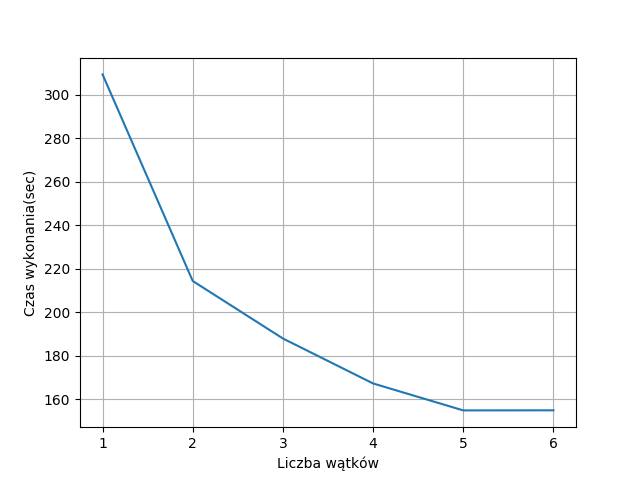
\includegraphics[width=0.6\textwidth]{img/plot_regular_threads_100x100.png}
    \caption{Zależność czasu wykonania programu od ilości używanych wątków dla modelu klasycznego dla zadania rozmiaru $100\times100$.}
    \label{threads_regular_100x100}
\end{figure}

\begin{figure}[H]
    \centering        
    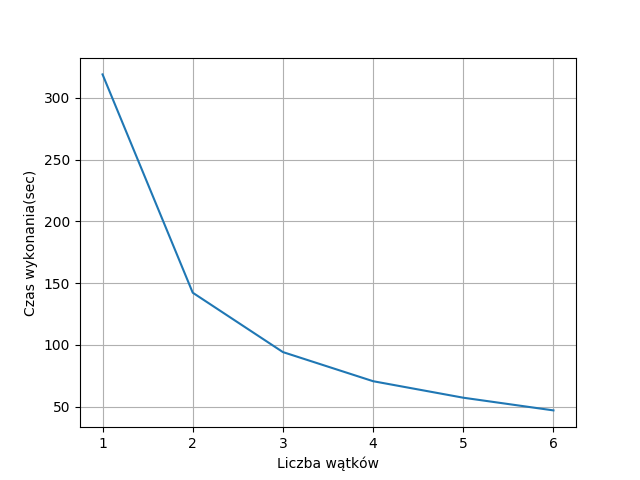
\includegraphics[width=0.6\textwidth]{img/plot_island_threads_100x100.png}
    \caption{Zależność czasu wykonania programu od ilości używanych wątków dla modelu wyspowego dla zadania rozmiaru $100\times100$.}
    \label{threads_island_100x100}
\end{figure}

\begin{figure}[H]
    \centering        
    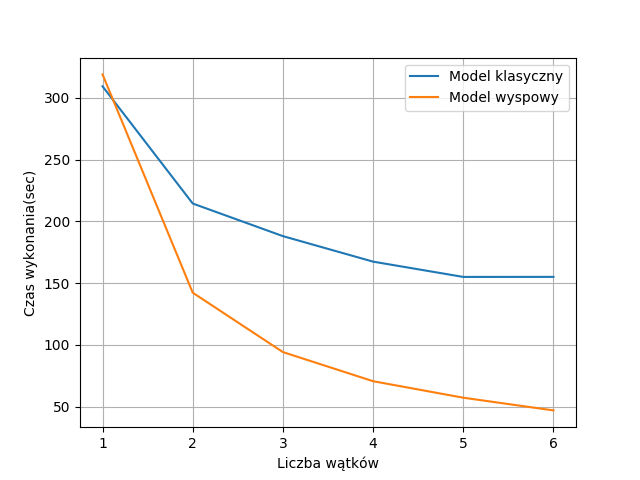
\includegraphics[width=0.6\textwidth]{img/plot_compare_threads_100x100.png}
    \caption{Porównanie modeli klasycznego i wyspowego pod względem zależności czasu wykonania programu od ilości używanych wątków dla zadania 
    rozmiaru $100\times100$.}
    \label{threads_comparsion_100x100}
\end{figure}

Możemy zauważyć, że spadek czasu wykonania jest dużo większy w przypadku modelu wyspowego (wykres \ref{threads_comparsion_100x100}). 
Wynika to z tego, że rozmiar zadania przydzielanego wątkom 
jest dużo większy w modelu wyspowym, niż w modelu klasycznym. Wprowadza on jednak dodatkowy warunek, czyli odpowiednio większą populacje. To znaczy, że 
im więcej wątków angażujemy, tym większa powinna być populacja całkowita, ponieważ jest ona rozdzielana na równe części, na przykład dla populacji 50 
osobników uruchomienie 10 wątków nie miałoby sensu z uwagi na to, że każdy działałby na 5 osobnikach. Skutkowałoby to bardzo szybką zbieżnością algorytmu, 
a co za tym idzie słabej jakości wynikami. Przykład pokazano na wykresie \ref{zla_zbieznosc_watki}. Uruchomiono model wyspowy z całkowitą populacją 40 osobników 
dla 2, 4 i 8 wątków. Wykres przedstawia ewolucje kosztu najlepszego osobnika na przestrzeni 10000 pokoleń.

\begin{figure}[H]
    \centering        
    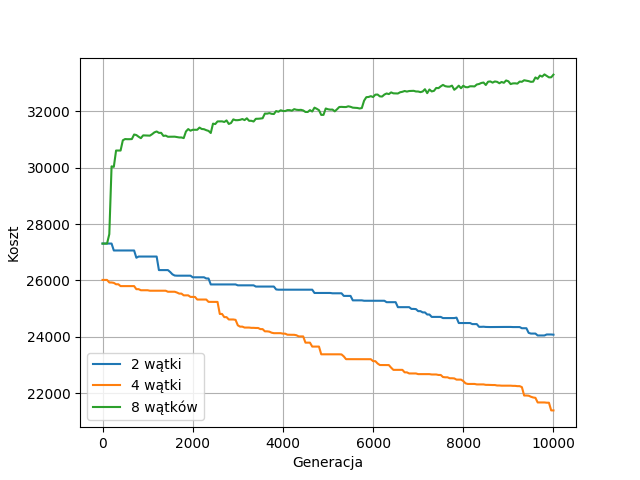
\includegraphics[width=0.6\textwidth]{img/zla_zbieznosc_watki.png}
    \caption{Ewolucja populacji 40 osobników dla 2, 4 i 8 populacji częściowych.}
    \label{zla_zbieznosc_watki}
\end{figure}

Widzimy tutaj, że w przypadku zastosowania 8 populacji częściowych koszt zamiast maleć na przestrzeni pokoleń, rośnie. Pokazuje to, że odpowiednio 
duży rozmiar populacji jest wymagany, aby algorytm ewolucyjny działał poprawnie.

Używanie dużej ilości wątków w przypadku modelu klasycznego ma sens podczas rozwiązywania bardzo dużych zadań. W mniejszych problemach dodatkowy narzut w 
postaci podziału zadań, komunikacji oraz synchronizacji jest większy niż zysk płynący z równoległości, przez co podniesienie ilości używanych wątków ponad 
określoną liczbę skutkuje zwiększeniem czasu potrzebnego na znalezienie rozwiązania. 

W celu lepszego pokazania jak rozmiar zadania wpływa na spadek czasu potrzebnego do zakończenia obliczeń wraz z dodaniem kolejnych wątków, wygenerowano 
dwa dodatkowe zadania rozmiaru $500 \times 500$ oraz $1000 \times 1000$. Następnie zmierzono czas obliczeń używając od 1 do 25 wątków. Dla większej 
przejrzystości przeskalowano wyniki w taki sposób, żeby oś y określała stosunek czasu obliczeń, do czasu potrzebnego przy użyciu 1 wątku. Rezultat 
pokazano na wykresie \ref{threads_comparsion_500x500_1000x1000}

\begin{figure}[H]
    \centering        
    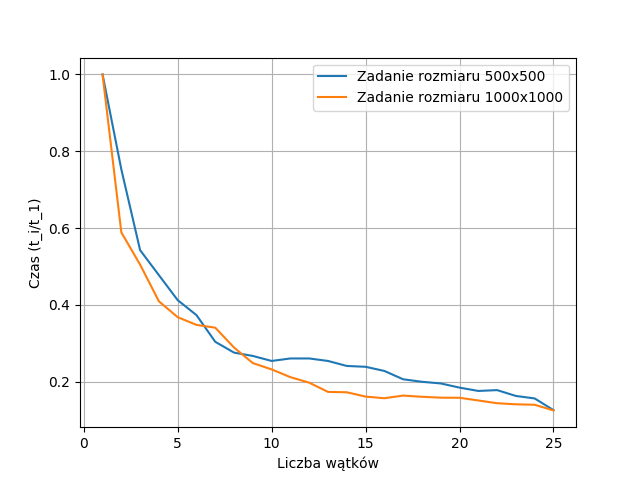
\includegraphics[width=0.6\textwidth]{img/compare_500_1000.png}
    \caption{Porównanie czasu dla zadań rozmiaru $500 \times 500$ i $1000 \times 1000$.}
    \label{threads_comparsion_500x500_1000x1000}
\end{figure}

Widzimy, że w przypadku większego zadania spadek czasu był większy wraz z dokładaniem kolejnych wątków, niż w przypadku mniejszego zadania. Dzieje się 
tak, ponieważ większe zadania przydzielane poszczególnym wątkom wydłużają czas współbieżnego działania aplikacji, jednocześnie nie zmieniając czasu
potrzebnego na synchronizację. Barierą, której nie jesteśmy jednak w stanie przeskoczyć 
są fragmenty kodu, które nie pozwalają się zrównoleglić oraz dodatkowy czas, którego potrzebuje garbage collector Julii na zarządzanie dostępną pamięcią. 
Wynikiem tego jest wypłaszczenie wykresu w miarę wzrostu wartości na osi x.

Porównując oba modele możemy dojść do wniosku, że algorytm wykorzystujący model wyspowy jest lepszy niż model klasyczny. Większe prawdopodobieństwo 
na znalezienie dobrego rozwiązania zapewnia nam użycie kilku niezależnych od siebie populacji częściowych. Dodatkowo zysk czasu jaki otrzymujemy 
przy użyciu dodatkowych wątków jest większy, nawet przy małych rozmiarach zadania. Jedynym minusem jest wymóg w postaci odpowiednio większej 
populacji dla tego modelu. 
	\cleardoublepage
	
	% % \chapter{Wyniki eksperymentalne}
% \thispagestyle{chapterBeginStyle}


% \section{}
	% \cleardoublepage
	
	\chapter{Podsumowanie}
\thispagestyle{chapterBeginStyle}

W tym rozdziale znajdzie się podsumowanie pracy.

% W podsumowanie należy określić stan zakończonych prac projektowych i implementacyjnych. Zaznaczyć, które z zakładanych funkcjonalności systemu udało się zrealizować. Omówić aspekty pielęgnacji systemu w środowisku wdrożeniowym. Wskazać dalsze możliwe kierunki rozwoju systemu, np.\ dodawanie nowych komponentów realizujących nowe funkcje.

% W podsumowaniu należy podkreślić nowatorskie rozwiązania zastosowane w projekcie i implementacji (niebanalne algorytmy, nowe technologie, itp.).




	\cleardoublepage
	
	
	%%%%%%%%%%%%%%%%%%%%%%%%%%%%%%%%%%%%%%%%%%%%%%%%%%%%%%%%%%%%%%%%%%%%%%%%%%%%%%
	%%%%%%%%%%%%%%%%%%%%%%%%%%%%%%% BIBLIOGRAFIA %%%%%%%%%%%%%%%%%%%%%%%%%%%%%%%%%
	%%%%%%%%%%%%%%%%%%%%%%%%%%%%%%%%%%%%%%%%%%%%%%%%%%%%%%%%%%%%%%%%%%%%%%%%%%%%%%

	\pagestyle{bibliographyStyle}
	\bibliographystyle{plabbrv}
	\bibliography{literatura}
	\thispagestyle{chapterBeginStyle}
        \addcontentsline{toc}{chapter}{Bibliografia}

	\cleardoublepage
	
	%%%%%%%%%%%%%%%%%%%%%%%%%%%%%%%%%%%%%%%%%%%%%%%%%%%%%%%%%%%%%%%%%%%%%%%%%%%%%%
	%%%%%%%%%%%%%%%%%%%%%%%%%%%%%%%%% DODATKI %%%%%%%%%%%%%%%%%%%%%%%%%%%%%%%%%%%%
	%%%%%%%%%%%%%%%%%%%%%%%%%%%%%%%%%%%%%%%%%%%%%%%%%%%%%%%%%%%%%%%%%%%%%%%%%%%%%%
	
	\appendix
	\pagestyle{appendixStyle}
	
	\chapter{Zawartość płyty CD}
\thispagestyle{chapterBeginStyle}
\label{plytaCD}

\section{Wymagania i instalacja}

Opisywany w poprzednich rozdziałach algorytm został zaimplementowany w języku Julia w wersji 1.3 oraz przetestowany na komputerze z zainstalowanym 
systemem Ubuntu 18.04 w wersji, dla architektury 64-bitowej. Prezentowany pakiet powinien jednak działać na każdym systemie, na którym 
Julia 1.3 działa poprawnie.

Dodatkowo pakiet wymaga zainstalowanych następujących bibliotek:

\begin{itemize}
    \item Random
    \item JSON
    \item PyPlot
    \item Distributions
    \item JuMP(skrypt \textit{optimizers.jl})
\end{itemize}

W przypadku, jeśli wymagane biblioteki nie są zainstalowane należy otworzyć \textit{REPL} Julii i przy pomocy modułu \textit{Pkg} dodać wymagane 
biblioteki poprzez wywołanie funkcji \textit{Pkg.add()}, gdzie w argumencie podajemy nazwę instalowanego pakietu, np:

\begin{lstlisting}
    Pkg.add("Distributions")
\end{lstlisting}

Po zainstalowaniu wyżej wymienionych zależności, biblioteka jest gotowa do użytku. Instrukcja obsługi została zamieszczona w kolejnych sekcjach.
Udostępniony pakiet zawiera zestaw testów jednostkowych, które weryfikują poprawność działania składowych algorytmu. Dodatkowo załączono przykładowy 
plik konfiguracyjny oraz definicje kilku funkcji kosztu.

W katalogu głównym znajdują się 3 foldery:

\begin{itemize}
    \item \textbf{src} - zawiera implementacje opisywanego algorytmu
    \item \textbf{tests} - zawiera testy jednostkowe
    \item \textbf{examples} - zawiera przykładowe pliki konfiguracyjne
\end{itemize}

W katalogu \textbf{src} znajdują się pliki:

\begin{itemize}
    \item \textbf{chromosom.jl} - zawiera definicje struktury reprezentującej pojedynczego osobnika w populacji. Znajdują się tutaj też wszystkie 
        funkcje operujące na zdefiniowanej strukturze takie jak operatory mutacji, krzyżowania, inicjalizacja, walidacja rozwiązania.
    \item \textbf{population.jl} - zawiera definicje struktury reprezentującej całą populację rozwiązań. Znajdują się tutaj wszystkie główne 
        funkcje operujące na populacji.
    \item \textbf{config.jl} - zawiera definicje struktury pliku konfiguracyjnego. Znajdują się tutaj funkcje odpowiedzialne za zapisywanie i wczytywanie 
        pliku konfiguracyjnego.
    \item \textbf{functions.jl} - w tym pliku znajdują się definicje wszystkich dostępnych funkcji celu. Każda taka funkcja powinna przyjmować 
        jeden argument typu \textit{Array\{Float64, 2\}}. Zdefiniowano tutaj też słownik, który mapuje nazwy funkcji do ich implementacji. Aby dodać 
        nową funkcje celu, użytkownik powinien zaimplementować ją w tym pliku, a następnie przypisać ją do konkretnej nazwy w słowniku.
    \item \textbf{GeneticNTP.jl} - zawiera definicje całego modułu o nazwie \textit{GeneticNTP}.
\end{itemize}

Dodatkowo w katalogu głównym znajduje się pliki:
\begin{itemize}
    \item \textit{run\_example.jl} - uruchamia przykładowe zadanie transportowe. Komentarze w pliku opisują krok po kroku jak używać algorytmu 
        korzystając z \textit{REPL} Julii.
    \item \textit{run.jl} - umożliwia uruchomienie programu dla dowolnego pliku konfiguracyjnego za pomocą polecenia:
    \begin{lstlisting}[language=bash]
$ julia run.jl plik_konfiguracyjny ilość_pokoleń nazwa_funkcji_kosztu
    \end{lstlisting}
    \item \textit{optimizers.jl} - umożliwia optymalizacje zadania transportowego z użyciem solverów \textbf{GLPK, Ipopt} i \textbf{CPLEX}. 
        Używa biblioteki JuMP w celu uruchomienia sloverów.
    \item \textit{configToGams.jl} - umożliwia konwersje pliku konfiguracyjnego na plik wejściowy GAMS.
\end{itemize} 

Przykładowe uruchomienie skryptu \textit{run\_example.jl}:

\begin{lstlisting}[language=bash, frame=single]
piotr@piotr-hp:~/geneticNTP$ julia run_example.jl 
Path: ./examples/ex_7x7.json
Running on 1 threads
==================== CONFIG ====================
Population Size: 100
Crossover: 70.0%
Mutation: 10.0% / rate: 0.05
Elite: 30.0%
Iterations: 10000
Cost Func: A

Best result in first generation: 1186.0
Best result: 201.0
\end{lstlisting}

Przykładowe uruchomienie skryptu \textit{optimizers.jl}:

\begin{lstlisting}[language=bash, frame=single]
piotr@piotr-hp:~$ julia optimizers.jl ./examples/ex_7x7.json GLPK Linear
START
Config loaded.
Using GLPK...
DONE.
Status: OPTIMAL
Result: 1132.0
\end{lstlisting}

\section{Pliki konfiguracyjne}

Do biblioteki został dodany moduł obsługi plików konfiguracyjnych. Używają one formatu JSON. Moduł pozwala na zapisywanie i wczytywanie 
całej konfiguracji algorytmu, w skład której wchodzą wektory popytu i podaży, macierz kosztu, oraz wszystkie parametry programu.
Definicja poszczególnych parametrów:

\begin{itemize}
    \item $populationSize$ - rozmiar całkowitej populacji. Powinien być dodatnią liczbą całkowitą.
    \item $eliteProc$ - ułamek najlepszych rozwiązań, które zostają przepisane do następnego pokolenia. 
    Wartość powinna znajdować się w przedziale $[0, 1]$. Testy pokazują, że najlepsze rozwiązania są generowane dla wartości parametru w przedziale
    $[0.1, 0.3]$.
    \item $mutationProb$ - prawdopodobieństwo mutacji. Przyjmuje wartość z zakresu $[0, 1]$. Warto pamiętać o tym, że zalecane prawdopodobieństwo 
    mutacji nie powinno przekraczać kilkanastu procent.
    \item $mutationRate$ - wielkość mutacji, określa stosunek rozmiaru podmacierzy, wybieranej do ponownej inicjalizacji podczas mutacji, 
    do macierzy rozwiązania. Przyjmuje wartości z zakresu $[0, 1]$. Tak jak w przypadku prawdopodobieństwa mutacji, jej wielkość nie powinna 
    przekraczać kilkunastu procent, ponieważ zbyt duża mutacja może niszczyć znalezione rozwiązania.
    \item $crossoverProb$ - prawdopodobieństwo krzyżowania. Przyjmuje wartości z przedziału $[0, 1]$. Zaleca się ustawialnie wartości z przedziału 
    $[0.5, 0.9]$. Należy pamiętać o tym, że suma parametrów eliteProc i crossoverProb nie może być większa niż $1$.
    \item mode - tryb w jakim ma działać algorytm. Przyjmuje wartości $regular$(w przypadku wyboru klasycznego modelu) lub $island$(w przypadku 
    modelu wyspowego).
    \item $numberOfSeparateGenerations$ - liczba naturalna określająca ilość iteracji jakie wykona algorytm pomiędzy rozdzieleniem populacji na 
    mniejsze części, a ponownym jej scaleniem. Dla wyboru modelu klasycznego należy ustawić wartość parametru na $1$.
\end{itemize}

Dodatkowo w pliku konfiguracyjnym określamy wektor popytu, podaży i macierz kosztów:

\begin{itemize}
    \item $demand$ - wektor popytu. Przyjmuje jako wartość listę elementów, które składają się z dwóch pól - $i$, które określa indeks wektora i 
    $val$, które określa wartosć wektora w miejscu $i$ - $demand[i] = val$.
    \item $supply$ - wektor podaży. Przyjmuje jako wartość listę elementów, o polach takich samych jak w przypadku wektora popytu. Pojedynczy element 
    opisuje pole wektora $supply[i] = val$.
    \item $costMatrix$ - macierz kosztu, która może być wykorzystywana w funkcji celu. Przyjmuje jako wartość listę elementów, które składają się 
    z trzech pól: $s$ - określa indeks odpowiadający indeksowi wektora podaży, $d$ - określa indeks odpowiadający indeksowi wektora popytu, oraz 
    $val$ - określa wartość macierzy w polu o podanych indeksach $costMatrix[d, s] = val$.
\end{itemize}

Przykładowy plik konfiguracyjny:

\begin{lstlisting}[language=json, firstnumber=1, frame=single]
{
    "populationSize": 100,
    "eliteProc": 0.3,
    "mutationProb": 0.1,
    "mutationRate": 0.05,
    "crossoverProb": 0.2,
    "mode": "regular",
    "numberOfSeparateGenerations": 1,
    "demand": [
        {
            "val": 1.0,
            "i": 1
        },
        {
            "val": 10.0,
            "i": 2
        }
    ],
    "supply": [
        {
            "val": 1.0,
            "i": 1
        },
        {
            "val": 5.0,
            "i": 2
        },
        {
            "val": 5.0,
            "i": 3
        }
    ],
    "costMatrix": [
        {
            "val": 1.0,
            "s": 1,
            "d": 1
        },
        {
            "val": 2.0,
            "s": 2,
            "d": 1
        },
        {
            "val": 3.0,
            "s": 3,
            "d": 1
        },
        {
            "val": 10.0,
            "s": 1,
            "d": 2
        },
        {
            "val": 20.0,
            "s": 2,
            "d": 2
        },
        {
            "val": 30.0,
            "s": 3,
            "d": 2
        }
    ]
}
\end{lstlisting}

\section{Uruchomienie biblioteki}

Przed uruchomieniem biblioteki należy zdefiniować w pliku \textit{functions.jl} funkcję kosztu dla zadania transportowego, lub skorzystać z 
wcześniej zdefiniowanych funkcji znajdujących się już w tym pliku. Następnie musimy stworzyć plik konfiguracyjny, według opisu znajdującego 
się w poprzedniej sekcji.

W celu uruchomienia biblioteki możemy używać przygotowanego skryptu znajdującego się w pliku \textit{run.jl}. Uruchamiamy go poprzez wywołanie 
interpretera Julii z argumentami:
\begin{enumerate}
    \item ścieżka do pliku \textit{run.jl}
    \item ścieżka do pliku konfiguracyjnego 
    \item maksymalna ilość pokoleń
    \item nazwa funkcji kosztu
\end{enumerate}

Przykład uruchomienia pliku:

\begin{lstlisting}[language=bash, frame=single]
piotr@piotr-hp:~/geneticNTP$ julia run.jl ./examples/ex_7x7.json 1000 B
Path: ./examples/ex_7x7.json
Running on 4 threads
==================== CONFIG ====================
Population Size: 100
Crossover: 70.0%
Mutation: 10.0% / rate: 0.05
Elite: 30.0%
Iterations: 1000
Cost Func: B

Best result in first generation: 660.8
Done in: 0.52914400100708 s
Best result: 265.8226422107641
\end{lstlisting}

W przypadku, jeśli chcielibyśmy używać biblioteki z poziomu \textit{REPL} Julii musimy wykonać następujące kroki:

\begin{enumerate}
    \item Włączamy \textit{REPL} Julii.
\begin{lstlisting}[language=bash, frame=single]
piotr@piotr-hp:~$ julia 
               _
   _       _ _(_)_     |  Documentation: https://docs.julialang.org
  (_)     | (_) (_)    |
   _ _   _| |_  __ _   |  Type "?" for help, "]?" for Pkg help.
  | | | | | | |/ _` |  |
  | | |_| | | | (_| |  |  Version 1.3.0 (2019-11-26)
 _/ |\__'_|_|_|\__'_|  |  Official https://julialang.org/ release
|__/                   |

julia> 

\end{lstlisting}

    \item Dołączamy bibliotekę \textit{GeneticNTP}.
\begin{lstlisting}[language=bash, frame=single]
julia> include("GeneticNTP.jl")
Main.GeneticNTP

julia> using .GeneticNTP
\end{lstlisting}

    \item Uruchamiamy algorytm wywołując funkcję \textit{runEA()}, gdzie w argumentach podajemy ścieżkę do pliku konfiguracyjnego, 
        maksymalną ilość pokoleń oraz nazwę funkcji kosztu z słownika znajdującego się w pliku \textit{functions.jl}
\begin{lstlisting}[language=bash, frame=single]
julia> c = GeneticNTP.runEA("../examples/ex_7x7.json", 1000, "A")
==================== CONFIG ====================
Population Size: 100
Crossover: 70.0%
Mutation: 10.0% / rate: 0.05
Elite: 30.0%
Iterations: 1000
Cost Func: A

Best result in first generation: 643.0    
\end{lstlisting}

    \item Wynikiem jest obiekt \textit{Chromosom}, który w polu \textit{result} posiada macierz rozwiązania, a w polu \textit{cost} koszt 
    znalezionego rozwiązania.
    
\begin{lstlisting}[language=bash, frame=single]
julia> c.result
7 x 7 Array{Float64,2}:
18.0516   0.386976  0.424021  0.285102  0.235168  0.273782  0.34338 
0.674536  16.1462   0.463446  0.999492  0.509193  0.40339   0.80372 
1.50289   1.54443   14.8906   0.809828  0.317118  0.306721  0.628409
1.90339   1.74331   3.83536   12.4525   0.0       1.31811   1.74737 
1.72222   1.47616   1.70419   3.91253   16.5287   0.391483  0.26473 
1.75765   1.10214   1.68994   0.975765  1.53068   16.6977   1.24612 
1.38773   5.60076   1.99244   0.564831  0.879151  0.608813  14.9663 

julia> c.cost
183.0

\end{lstlisting}

\end{enumerate}


	\cleardoublepage

\end{document}

